%-----------------------------------------------------------------
% Link do repozitorijuma na pltaformi GitHub: https://github.com/PosteruOle/master_thesis
%-----------------------------------------------------------------
% Format teze zasnovan je na paketu memoir
% http://tug.ctan.org/macros/latex/contrib/memoir/memman.pdf ili
% http://texdoc.net/texmf-dist/doc/latex/memoir/memman.pdf
% 
% Prilikom zadavanja klase memoir, navedenim opcijama se podešava 
% veličina slova (12pt) i jednostrano štampanje (oneside).
% Ove parametre možete menjati samo ako pravite nezvanične verzije
% mastera za privatnu upotrebu (na primer, u b5 varijanti ima smisla 
% smanjiti 
\documentclass[12pt,oneside]{memoir}

% Paket koji definiše sve specifičnosti mastera Matematičkog fakulteta
\usepackage[latinica]{matfmaster}
%
% Podrazumevano pismo je ćirilica.
%   Ako koristite pdflatex, a ne xetex, sav latinički tekst na srpskom jeziku
%   treba biti okružen sa \lat{...} ili \begin{latinica}...\end{latinica}.
%
% Opicija [latinica]:
%   ako želite da pišete latiniciom, dodajte opciju "latinica" tj.
%   prethodni paket uključite pomoću: \usepackage[latinica]{matfmaster}.
%   Ako koristite pdflatex, a ne xetex, sav ćirilički tekst treba biti
%   okružen sa \cir{...} ili \begin{cirilica}...\end{cirilica}.
%
% Opcija [biblatex]:
%   ako želite da koristite reference na više jezika i umesto paketa
%   bibtex da koristite BibLaTeX/Biber, dodajte opciju "biblatex" tj.
%   prethodni paket uključite pomoću: \usepackage[biblatex]{matfmaster}
%
% Opcija [b5paper]:
%   ako želite da napravite verziju teze u manjem (b5) formatu, navedite
%   opciju "b5paper", tj. prethodni paket uključite pomoću: 
%   \usepackage[b5paper]{matfmaster}. Tada ima smisla razmisliti o promeni
%   veličine slova (izmenom opcije 12pt na 11pt u \documentclass{memoir}).
%
% Naravno, opcije je moguće kombinovati.
% Npr. \usepackage[b5paper,biblatex]{matfmaster}

% Pomoćni paket koji generiše nasumičan tekst u kojem se javljaju sva slova
% azbuke (nema potrebe koristiti ovo u pravim disertacijama)
\usepackage{pangrami}
\usepackage{graphicx}
\usepackage{minted}
\graphicspath{ {./assets/} }

% Paket koji obezbeđuje ispravni prikaz ćiriličkih italik slova kada
% se koristi pdflatex. Zakomentarisati ako na sistemu koji koristite ovaj
% paket nije dostupan ili ako ne radi ispravno.
\usepackage{cmsrb}

% Ostali paketi koji se koriste u dokumentu
\usepackage{listings} % listing programskog koda

% Datoteka sa literaturom u BibTex tj. BibLaTeX/Biber formatu
\bib{PetarTesicMasterRad}

% Ime kandidata na srpskom jeziku (u odabranom pismu)
\autor{Petar Tešić}
% Naslov teze na srpskom jeziku (u odabranom pismu)
\naslov{Automatska detekcija i optimizacija algoritma CRC u okviru kompajlerske infrastrukture LLVM}
% Godina u kojoj je teza predana komisiji
\godina{2024}
% Ime i afilijacija mentora (u odabranom pismu)
\mentor{dr Milena Vujošević Janičić, vanredni profesor\\ Univerzitet u Beogradu, Matematički fakultet}
% Ime i afilijacija prvog člana komisije (u odabranom pismu)
\komisijaA{dr Filip Marić, vanredni profesor\\ Univerzitet u Beogradu, Matematički fakultet}
% Ime i afilijacija drugog člana komisije (u odabranom pismu)
\komisijaB{dr Mirko Spasić, docent\\ Univerzitet u Beogradu, Matematički fakultet}
% Ime i afilijacija trećeg člana komisije (opciono)
% \komisijaC{}
% Ime i afilijacija četvrtog člana komisije (opciono)
% \komisijaD{}
% Datum odbrane (obrisati ili iskomentarisati narednu liniju ako datum odbrane nije poznat)
\datumodbrane{21. jun 2024.}

% Apstrakt na srpskom jeziku (u odabranom pismu)
\apstr{
U savremenoj industriji razvoja softvera, efikasnost i optimizacija koda predstavljaju ključne 
aspekte u postizanju visokih performansi računarskih sistema. Ovaj master rad istražuje 
inovativan pristup prevođenju algoritma CRC (engl. Cyclic Redundancy Check) u kontekstu 
različitih procesorskih arhitektura, a specijalno i u kontektstu procesorske arhitekture RISC-V, 
korišćenjem kompajlerske infrastrukture LLVM.

Motivacija za ovu istraživačku oblast proizlazi iz široke primene CRC algoritma u digitalnoj 
komunikaciji, u kojoj se ovaj algoritam često koristi za proveru integriteta podataka. 
Identifikacija neoptimizovanih verzija CRC algoritma i zamenjivanje semantički im ekvivalentnim 
optimizovanim verzijama na različitim procesorskim arhitekturama, pa i na arhitekturi RISC-V, ima 
potencijal da značajno poboljša efikasnost i performanse ugrađenih sistema i drugih aplikacija 
koji koriste ovaj algoritam.

Prvi deo rada posvećen je predstavljanju fundamentalnih znanja o procesu prevođenja programa, 
arhitekturi modernih kompilatora, kao i o projektu LLVM. Drugi deo ovog rada posvećen je analizi 
CRC algoritma i problema njegovog prepoznavanja u postojećem kodu, korišćenjem različitih 
biblioteka u okviru projekta LLVM. Nakon detekcije CRC algoritma, pažnja se usmerava ka 
optimizaciji koda na nivou LLVM međureprezentacije, kao i  u drugim fazama prevođenja programa. 

Cilj ovog rada je unapređivanje LLVM infrastrukture u kontekstu efikasnijeg prevođenja CRC 
algoritma, a samim tim i performansi programa koji koriste CRC algoritam i LLVM kao svoj 
kompajler. Unapređenje bi trebalo da bude vidljivo na različitim procesorskim arhitekturama, 
specijalno i na arhitekturi RISC-V, ali da pritom održi primarnu svrhu CRC algoritma, a to je 
čuvanje integriteta podataka. Rezultati dobijeni testiranjem rešenja predstavljenog u ovom radu 
pokazuju značajno poboljšanje performansi CRC algoritma prevedenog LLVM kompilatorom.
}

% Ključne reči na srpskom jeziku (u odabranom pismu)
\kljucnereci{LLVM, CRC, RISC-V, IR, MIR, TableGen, LLVM pass}

\begin{document}
% ==============================================================================
% Uvodni deo teze
\frontmatter
% ==============================================================================
% Naslovna strana
\naslovna
% Strana sa podacima o mentoru i članovima komisije
\komisija
% Strana sa posvetom (u odabranom pismu)
\posveta{Zahvaljujem se svojoj porodici, prijateljima, Kaći, profesorki Mileni i svim kolegama iz kompanije SYRMIA na nesebičnoj pomoći i podršci}
% Strana sa podacima o disertaciji na srpskom jeziku
\apstrakt
% Sadržaj teze
\tableofcontents*

% ==============================================================================
% Glavni deo teze
\mainmatter
% ==============================================================================

% ------------------------------------------------------------------------------
\chapter{Uvod}
% ------------------------------------------------------------------------------
Iako je u industriji razvoja softvera najčešće sva pažnja i energija usmerena 
ka izvornom kodu projekata i rezultatima koji taj isti projekat proizvodi tokom 
svog izvršavanja, ne smemo zanemariti bitnost programskih prevodilaca koji te projekte prevode u što kvalitetniji mašinski kod i time zapravo omogućavaju njihovo izvršavanje na različitim arhitekturama računara. Ove činjenice je veliki broj softverskih korporacija i svestan i stoga veliku količinu finansijskih sredstava ulaže u njihov razvoj sa ciljem da njihovi proizvodi ostanu konkurentni na svom tržištu.

Rivalitet između različitih programskih prevodilaca odnosno kompilatora...

Politika unapređivanja kompilatora tako da se izvorni kod što više optimizuje kako bi se od istog dobio što optimalniji mašinski kod...

Ovaj rad se sastoji od pet poglavlja. U drugom poglavlju se govori uopšteno o procesu prevođenja programa, metodologijama konstrukcije kompilatora i na kraju o kompilatorskoj infrastrukturi LLVM.
U okviru sekcije posvećenoj LLVM-u govori se o istoriji samog projekta, njegovoj arhitekturi, malo detaljnije o svakom od delova LLVM kompilatora (prednjem, srednjem i zadnjem delu). Poslednja sekcija drugog poglavlja posvećena je LLVM međureprezentaciji, kako bi objašnjenje 
implementacije rešenja bilo što razumljivije.

Treće poglavlje je posvećeno algoritmu CRC i problemu njegovog prepoznavanja. 

Četvrto poglavlje je posvećeno procesorskim arhitektura, a specijalno i procesorskoj arhitekturi RISC-V.

Peto poglavlje bi trebalo da predstavi način na koji su oba rešenja problema implementirana.

Šesto poglavlja će predstaviti rezultate do kojih se došlo pokretanjem rešenja predstavljenih u prethodnom poglavlju.
% ------------------------------------------------------------------------------
\chapter{Kompilatori i projekat LLVM}
\section{Faze prevođenja programa}
% ------------------------------------------------------------------------------
Krajnji cilj kreiranja svakog softvera jeste njegovo izvršavanje na računaru. 
Kako bi se tako nešto postiglo, potrebno je da se nad programom napisanim na 
višem programskom jeziku sprovede ili proces kompilacije ili proces 
interpretacije. U zavisnosti od toga za koji od ova dva procesa se opredelite 
(zapravo koji programski jezik odaberete) koristićete ili 
kompilator (odnosno kompajler) ili interpreter.

Proces kompilacije podrazumeva korišćenje programa koji zovemo kompilator, a 
koji garantuje razdvojenost procesa prevođenja i procesa izvršavanja našeg 
programa. Kompilacijom se može kreirati izvršiva datoteka koju je potom moguće pokretati, to 
jest, izvršavati na računaru proizvoljan broj puta. Za svaku promenu u izvornom kodu potrebno je 
ponoviti proces kompilacije. Neki od najpoznatijih kompilatora danas su GCC, LLVM, RUSTC, GraalVM 
i drugi. Programski jezici za čije prevođenje je potrebno koristiti kompilaciju su C, C++, Rust, 
Go i mnogi drugi.

\begin{figure}
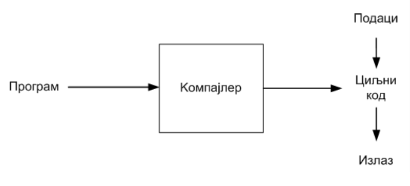
\includegraphics[width=\textwidth, height=6cm]{kompilacija}
\caption{Proces kompilacije}
\centering
\end{figure}

Prilikom procesa interpretacije faze prevođenja i izvršavanja programa su 
isprepletane. To znači da se interpretacijom svaka naredba prvo parsira, što znači da se, a potom se izvršava. Pod parsiranjem naredbe podrazumevamo proveru njene leksičke, sintaksne i semantičke ispravnosti. Bilo koja greška u programu (bilo leksička, bilo sintaksna, bilo semantička) biće otkrivena tek kada se parsiranjem dođe do linije u kojoj se ona nalazi. 

\begin{figure}
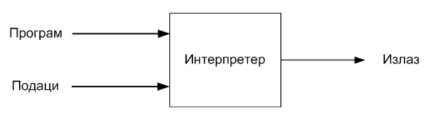
\includegraphics[width=\textwidth, height=5cm]{interpretacija}
\caption{Proces kompilacije}
\centering
\end{figure}

Na slici 2.1. prikazana je skica procesa kompilacije, dok je na slici 2.2. isto urađeno samo za proces interpretacije. U nastavku rada bilo kakvo ponovno spominjanje procesa prevođenja odnosiće se isključivo na kompilaciju.

U okviru procesa prevođenja programa postoje više različitih faza, a to su: leksička 
analiza, sintaksna analiza, semantička analiza, optimizacija i generisanje koda.
U fazi leksičke analize, za koju je odgovaran deo programskog prevodioca koji 
zovemo leksički analizator ili lekser, ustanovljava se da li su u izvornom kodu 
iskorišćene samo dopustive lekseme. Pod dopustivim leksemama podrazumevamo reči napisane u našem izvornom kodu koje mogu biti prepoznate jednim od unapred definisanih regularnih izraza. Pomenuti regularni izrazi imaju za cilj da opiši imena promenljivih, operatore, separatore i tako dalje. Ukoliko je program koji prevodimo sačinjen isključivo od dopustivih leksema, u tom slučaj niz prepoznatih 
leksema se prosleđuje, delu programskog prevodioca zaduženom za sintaksnu 
analizu, odnosno sintaksnom analizatoru iliti parseru. U protivnom, u slučaju 
detektovanja nedopustive lekseme, proces prevođenja se zaustavlja i programski 
prevodilac nam saopštava poruku o leksičkoj greški. 

%Dodatooooo
U narednoj fazi, fazi sintaksne analize, proverava se da li su prepoznate lekseme u skladu sa 
gramatikom programskog jezika u kome je izvorni kod napisan. 
Ta pravila se zadaju korišćenjem kontekstno-slobodne gramatike
(eng. context-free grammar). Primenom pravila gradi se stablo parsiranja (eng. parse
tree). Svaki unutrašnji čvor tog stabla predstavlja jednu operaciju, a njegova deca
predstavljaju argumente te operacije. U slučaju upotrebe nedozvoljene rečenične konstrukcije, proces prevođenja se zaustavlja i prevodilac nam saopštava poruku o sintaksnoj greški. Ukoliko do upravo pomenutih grešaka nije došlo, započinje se faza semantičke analize u kojoj se 
dodeljuje značenje ispravnim rečeničnim konstrukcijama. 

Dakle, sintaksnom analizom se utvrđuje da li program ima ispravnu
strukturu, ali se smisao tog programa ne proverava. To je zadatak semantičke
analize. Program može da ima dobru strukturu, ali da nema validno značenje. Prolaskom
kroz stablo parsiranja se prikupljaju informacije o funkcijama, promenljivima i dru-
gim objektima i smeštaju se u tabelu simbola. Korišćenjem te tabele proverava se
ispravnost stabla parsiranja. Primer provere koja se vrši na ovom nivou je da li su
promenljive deklarisane pre njihove upotrebe. Rezultat svih ovih analiza je program
u obliku apstraktnog sintaksnog stabla (eng. Abstract Syntax Tree, AST).

Preostale su još dve faze (optimizacija i generisanje koda) i one će upravo biti objašnjene.
Faza optimizacije se započinje nakon uspešno završene semantičke analize. Kao rezultat uspešne semantičke analize dobija se međukod izvornog programa nad kojim će se sprovesti faza optimizacije. Cilj ove faze jeste analiziranje i optimizovanje međukoda kako bi se od njega dobio što kvalitetniji mašinski kod. Faza generisanja koda je poslednja faza prevođenja u kojoj od optimizovanog međukoda dobija mašinski kod za odabranu odnosno ciljnu procesorsku arhitekturu.
Više o fazi optimizacije i generisanja koda biće reči u narednoj sekciji.

% ------------------------------------------------------------------------------
\section{Kompilatori}
% ------------------------------------------------------------------------------
Kompilatori iliti kompajleri predstavljaju veoma kompleksan softver sposoban da 
proizvoljan kod napisan u nekom višem programskom jeziku konvertuje u 
kvalitetan mašinski kod koji će se potom izvršavati na računaru. U arhitekturi 
većine današnjih kompilatora moguće je uočiti tri bitna dela odnosno celine.
U pitanju su prednji deo (front end), srednji deo (middle end) i zadnji deo (back end) kompilatora.

%Prednji deo kompilatora...
Prednji deo kompilatora je zavisan od višeg programskog jezika kojeg prevodi. Odgovornost prednjeg dela kompilatora jeste obavljanje leksičke, 
sintaksne i semantičke analize. Kao rezultat rada prednjeg dela kompilatora 
dobija se međureprezentacija (engl. intermediate representation) izvornog koda.
Za međureprezentaciju se može reći da je reprezentacija nižeg nivoa početnog 
programa. Rezultat prednjeg dela kompilatora se potom prosleđuje srednjem delu kompilatora.

%Srednji deo kompilatora...
Srednji deo kompilatora (middle end) je nezavisan od programskog jezika i ciljne arhitekture. Njegova odgovornost jeste sprovođenje optimizacija na međukodu (međureprezentaciji) kako bi se unapredile njegove performanse i kako bi se od istog dobio kvalitetan mašinski kod na samom kraju kompilacije. Srednji deo kompajlera izvršava optimizacije na međureprezentaciji koje su
nezavisne od CPU arhitekture za koju je krajnji kod namenjen. Može da radi u jednom ili više prolaza.

Da bi srednji deo kompajlera izvršio kvalitetnu optimizaciju, najpre vrši analizu koda.
Analiza obuhvata prikupljanje informacija o programu na osnovu generisane
međureprezentacije. Postoje razne vrste analiza, kao što su analiza toka podataka, analiza 
zavisnosti, analiza aliasa, analiza pointera i druge. Precizne analize su osnova za svaku 
kvalitetnu optimizaciju. U fazi analize koda, obično se grade i graf kontrole toka i graf poziva 
funkcija.

Koristeći rezultate analize, vrši se odgovarajuća optizacija.
Pod optimizacijom podrazumevamo transformisanje međureprezentacija u funkcionalno
ekvivalentan, ali brži ili manji oblik. Popularne optimizacije uključuju inline, eliminaciju mrtvog koda, propagiranje konstanti, transformaciju petlji, čak i neke vrste automatske paralelizacije. Izbor optimizacija koje će biti izvršene zavisi od želja korisnika i argumenata koji se zadaju prilikom pokretanja kompajlera. Podrazumevan nivo optimizacija obuhvata optimizacije nivoa -O2.

\begin{figure}
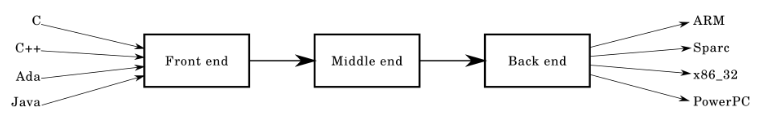
\includegraphics[width=\textwidth, height=4cm]{frontmidback}
\caption{Arhitektura modernih kompilatora}
\centering
\end{figure}

%Zadnji deo kompilatora...
Zadnji deo kompilatora (back end) zavisi od ciljne arhitekture i zadužen je za generisanje koda za ciljnu arhitekturu. Takođe je i odgovoran za arhitekturalno specifične optimizacije. Osnovne faze zadnjeg dela kompajlera obuhvataju arhitekturalno specifičnu optimizaciju i 
generisanje koda. Mašinski zavisne optimizacije podrazumevaju optimizacije koje zavise od detalja 
arhitekture procesora na kojem će se program izvršavati. Ove optimizacije 
obuhvataju, na primer prepisivanje kraćih nizova instrukcije u odovarajuće 
instrukcije koje su efikasnije.

Generisanje koda podrazumeva da se transformisan međukod translira u izlazni 
jezik, obično mašinski jezik računarskog sistema. Ovo uključuje odluke vezane 
za resurse i skladištenje podataka, kao na primer koje promenljive će biti u 
registrima a koje u memoriji, i izbor i odredivanje redosleda instrukcija 
zajedno sa odgovarajućim tipovima adresiranja. Takode, podaci za debagovanje 
treba da se generišu kako bi omogućili debagovanje.

Za generisanje mašinskog koda potrebni su samo prednji i zadnji deo kompilatora. Optimizator odnosno srednji deo je opcioni i nastao je iz potrebe da dobijeni kôd ima dobre preformanse. Svaki dobar kompajer ga ipak sadrži, i on čini jedan od najvećih delova kompilatora. Odnos
ovih delova je prikazan na slici 2.1. U svakom trenutku program je enkodiran u neku
vrstu interne reprezentacije. U svakom koraku, ta reprezentacija postaje sve bliža mašinskom kodu. Ovakva struktura omogućava lako dodavanje podrške za druge programske jezike kao i za nove arhitekture.

Neki od najpoznatijih kompilatora otvorenog koda su GCC, LLVM i GraalVM. U 
narednom poglavlju biće predstavljen i detaljnije objašnjen kompilator LLVM.

% ------------------------------------------------------------------------------
\section{Kompajlerske optimizacije}
% ------------------------------------------------------------------------------
Kao što je već spomenuto, kompilatori osim mogućnosti prevođenja izvornog koda u mašinski kod imaju, takođe, i mogućnosti modifikovanja istog (mašinskog koda) kako bi imao bolje performanse.
Jedini uslov koji pritom mora biti ispoštovan jeste da se optimizovani kod ponaša isto kao i originalni kod. Performanse mogu da se odnose na vreme izvršavanja programa,
memorijski prostor potreban prilikom izvršavanja ili memorijski prostor potreban za
skladištenje izvršnog fajla. U zavisnosti od faze kompilacije u kojoj se rade, optimi-
zacije mogu biti nezavisne ili zavisne od ciljne arhitekture. Nezavisne optimizacije
rade za sve ciljne arhitekture i oslanjaju se na smanjivanje ukupnog broja operaci-
ja koje treba izvršiti. Zavisne optimizacije iskorišćavaju detalje arhitekture kako bi
podigli performanse. To se ogleda u korišćenju instrukcija koje rade više operacija u
isto vreme, imaju kraći zapis ili rade brže od alternativa. Čest primer na arhitekturi
x86-64 je zamena instrukcije mov eax, 0 sa instrukcijom xor eax, eax. 
Prva instrukcija direktno postavlja vrednost registra eax na 0. Druga instrukcija radi isto
to, ali konstantu 0 dobija kao rezultat binarne ekskluzivne disjunkcije čija su oba
operanda vrednost registra eax. Obe operacije imaju isti ishod, ali druga zauzima
manje memorije i u nekim slučajevima se brže izvršava.

Optimizacije se u odnosu na opseg koda koji obrađuju mogu podeliti na: lokalne optimizacije, globalne optimizacije i interproceduralne optimizacije.
Lokalne optimizacije rade na nivou jednog osnovnog bloka (eng. basic block).
Ovo su najjednostavnije optimizacije zato što ne obrađuju instrukcije skoka.
Globalne (intraproceduralne) optimizacije operišu na nivou pojedinačnih
funkcija. Većina lokalnih optimizacija se može modifikovati da radi globalno.
Interproceduralne optimizacije rade na nivou čitavog programa. One isto-
vremeno obrađuju više funkcija, potencijalno iz različitih kompilacionih jedi-
nica.

Primeri za svaku od prethodnih grupa redom su: sažimanje konstanti, globalna numeracija vrednosi i umetanje koda.

Sažimanje konstanti (eng. constant folding) — U programskom kodu se često
javljaju konstantni matematički izrazi bez promenljivih. Oni mogu da budu
direkno napisani u izvornom kodu, dobijeni pretprocesiranjem ili drugim op-
timizacijama itd. Kako izraz ne sadrži promenljive, nema razloga da se on
izračunava za vreme izvršavanja svaki put, već se to radi u vreme kompilacije.

Globalna numeracija vrednosti (eng. global value numbering) — Neki izra-
zi ili delovi izraza se mogu pojaviti na više mesta u kratkom rasponu u okviru
funkcije. Ukoliko su izračunati jednom, nije potrebno računati ih ponovo is-
početka već je moguće obezbediti da prethodni rezultat ostane dostupan u
memoriji dok nije ponovo potreban.

Umetanje koda (eng. inlining) — Pozivi funkcija su skupa operacija zato što
menjaju kontrolu toka izvršavanja i zahtevaju dodatne instrukcije za čuvanje
i učitavanje vrednosti registara. Zbog toga je poželjno zameniti pozive kratkih
funkcija sa njihovom definicijom. Time se izbegava cena poziva o trošku veće
količine memorije za čuvanje programa.

Postoji nekoliko nivoa optimizacije koji se mogu podesiti prilikom poziva kom-
pilatora. Izbor nivoa određuje koje optimizacije treba da se izvrše. Način odabira i
nivoi optimizacije su drugačiji na različitim kompilatorima. Na kompilatorima gcc i
clang korisnik može da izabere nivo tako što prosledi zastavicu -O iza koje se javlja
neki od karaktera 0, 1, 2, 3 ili s1. O0 je podrazumevani nivo ukoliko nijedan drugi nije
naveden i označava da se kôd uopšte ne optimizuje. Ovaj režim se koristi za pravlje-
nje debag verzija programa. Više reči o tome će biti u poglavlju 3.1. O1 i O2 redom
uključuju sve veći broj optimizacija podrazumevano da one drastično ne povaćavaju
memorijsku složenost programa. O3 ja najveći nivo optimizacije vremena izvršava-
nja. On podrazumeva sve što se koristi u O2, ali uključuje i optimizacije koje mogu
da znatno povećaju memorijsko zauzeće programa. Isporučene verzije programa se
često kompiliraju na ovaj način. Sa druge strane Os nivo takođe podrazumeva sve
optimizacije iz O2 ali dodatno i optimizacije koje smanjuju memorijsko zauzeće na
uštrb vremena izvršavanja. Ovaj nivo se koristi za uređaje sa ugrađenim računarom
(eng. embedded devices) koji imaju malu količinu memorije.

% ------------------------------------------------------------------------------
\section{Kompajlerska infrastruktura LLVM}
% ------------------------------------------------------------------------------
Projekat LLVM je započet kao istraživački projekat 2000. godine na Univerzitetu 
Ilinois od strane Krisa Latnera, čoveka koga je ovaj projekat i proslavio, a koji danas radi na razvoju programskog jezika Mojo. 
Cilj projekta LLVM je bio proučavanje tehnika kompajliranja u SSA obliku (eng. 
Static Single Assignment). Naziv LLVM je predstavljao akronim za „virtuelna 
mašina niskog nivoa” (eng. Low Level Virtual Machine). Međutim, isti akronim se 
više ne koristi, ali je ime projekta ostalo nepromenjeno. Danas, projekat 
sadrži veliki broj biblioteka i alata koji se koriste kako u komercijalne svrhe 
tako i u svrhe razvoja projekata otvorenog koda. Svaki deo projekta je 
dizajniran kao biblioteka tako da se može ponovo upotrebiti za implementiranje 
drugih alata. 
Celokupan izvorni kôd je javno dostupan na servisu GitHub i oko njega je 
formirana velika zajednica ljudi koji rade na različitim delovima LLVM i 
svakodnevno ga unapređuju. Veliki broj kompanija koristi svoje verzije 
kompilatora LLVM bilo u celosti bilo samo neke njegove delove (prednji, srednji 
ili zadnji deo kimpilatora) za podršku neke procesorkse arhitekture ili kao 
osnovu za novi programski jezik. 

O popularnosti projekta LLVM govori i činjenica da se dva puta u toku svake 
godine organizuje LLVM Developers Meeting i LLVM WorkShop u različitim 
gradovima Evrope i Amerike. LLVM je dobio 2012 godine nagradu ACM Software System Award (nagrada se dodeljuje jednom softverskom sistemu godišnje, počevši od 1983. godine, gcc 
je dobio nagradu 2015. godine). Licenca koda u okviru LLVM projekta je ”Apache 2.0 License with LLVM exceptions”. Licenciranje se menjalo tokom razvoja projekta, ali je uvek bila licenca otvorenog koda.

Kao što je već rečeno, LLVM se sastoji od velikog broja manjih podprojekata 
koji predstavljaju zasebne i funkcionalne celine. Neki od tih primarnih projekata su 
LLVM Core Libraries, Clang, libc++, libc++ ABI, compiler-rt, MLIR, OpenMP, polly, klee, LLD, BOLT i drugi. Svi potprojekti zajedno čine potpun programski prevodilac koji ima
svoj prednji deo (eng. frontend), srednji deo (eng. middleend), zadnji deo
(eng. backend), optimizatore, asemblere, linkere i druge alate koji pružaju prodšku u čitavom procesu prevođenja koda na ciljnu arhitekturu. LLVM implementira i svoj
debager koji se zove LLDB.

Kompilator LLVM je relativno nov u odnosu na druge popularne kompilatore
i prati moderniji dizajn. Za razliku od kompilatora GCC, koji je napisan u
jeziku C i ima monolitnu strukturu, LLVM uživa u pogodnostima koje nudi jezik
C++ pritom koristeći modularnu arhitekturu. Dok je najveći deo projekta napisan u programskom jeziku C++, postoji interfejs za povezivanje sa jezicima C i Python.
Implementacija kompilatora LLVM prati opštu strukturu kompilatora prikazanu
u poglavlju 2.2. Korake kompilacije izvršavaju različiti alati. Odnos različitih
reprezentacija koje program ima u toku kompilacije i alata koji konvertuju iz jedne
reprezantacije u drugu je prikazan na slici 2.2. 
 
U nastavku će biti opisani redom prednji, srednji i zadnji deo kompilatora LLVM sa fokusom na poslednja dva kako su oni bitniji za ovaj rad.

%Prvi deo backend-a se bavi selekcijom instrukcija. Opšte IR instrukcije se prevode 
%u mašinske instrukcije za našu odabranu ciljnu arhitekturu. Odnosno IR se prevodi u 
%MIR. 

%Prednji deo LLVM-a!!!!
\subsection{Prednji deo LLVM-a}
Prednji deo LLVM kompilatora je zadužen za pokretanje leksičke, sintaksne i semantičke analize, kreiranje apstraktnog sintaksnog stabla i na kraju generisanja LLVM međukoda.
Kompilator LLVM podržava više različitih prednjih delova kompilatora. Mnoge organizacije i kompanije takođe razvijaju i održavaju prednje delove kompilatora LLVM za svoje jezike. Iz tog razloga, LLVM podržava veliki broj programskih jezika kao što su C, C++, Objectve-C, Fortran, Haskell, Swift i drugi. Prednji deo kompilatora prilagođen jezicima C i C++ koji su korišćeni u ovom radu jeste Clang. Termin Clang može imati više značenja. Clang može predstavljati prednji deo kompilatora, baš kao što smo to upravo spomenuli, zatim može predstavljati čitav kompilator (alat koji upravlja čitavim procesom kompilacije), a takođe može biti korišćen i kao biblioteka koja implementira funkcionalnosti prednjeg dela kompilatora. U okviru rada, termin Clang će od sada, pa na dalje, predstavljati prednji deo LLVM kompilatora.
Funkcija ovog dela kompilatora je da izvorni kôd, u ovom slučaju napisan u
jezicima C ili C++ prevede u LLVM međureprezentaciju. 
Naravno, da bi se tako nešto postiglo, potrebno je proveriti ispravnost izvornog koda i korisniku prikazati sve potencijalne greške i upozorenja. Program se u nekoliko koraka detaljno analizira, a potom dolazi do transformacija izvornog koda.

U biblioteci Clang parsiranje i semantička analiza su usko povezani, a lekser se
poziva po potrebi od strane parsera. Bitan korak koji se izvršava pre leksiranja
je pretprocesiranje u okviru kog se obrađuju direktive poput \#include i \#define.
Prilikom primene pravila gramatike parser zahteva tokene od leksera i delegira posao kreiranja sintaksnog stabla semantičkom analizatoru. Ukoliko se pronađe greška
u bilo kojoj analizi, program se ne moze kompilirati i poruka o razlogu se vraća korisniku. U suprotnom, obilaskom apstraktnog sintaksnog stabla generiše se LLVM
međukod. Komanda za prevođenje programa do LLVM međukoda je sledeća:
\begin{minted}[breaklines, fontsize=\small]{bash}
clang -S -emit-llvm -o output.ll input.c
\end{minted}

Ukoliko se program uspešno prevede do međukoda, onda je izvorni kôd validan za
jezik u kome je napisan. Još uvek je moguće da dođe do greške prilikom povezivanja
zbog nepostojećih definicija nekih funkcija, klasa ili simbola, ali će kompilacija do
asemblerskog ili objektnog koda biti uspešna.

%Srednji deo LLVM-a!!!!
\subsection{Srednji deo LLVM-a}
Srednji deo LLVM kompilatora zadužen je za sprovođenje mašinski nezavisnih optimizacija nad LLVM međureprezentacijom dobijenom od strane Clang-a. LLVM međukod je u SSA obliku. Ovaj oblik je izabran zato što je pogodan za izvršavanje optimizacija. Detaljniji opis jezika LLVM IR nalazi se u poglavlju 2.5.
Optimizacije su implementirane u vidu prolaza (eng. pass) koji obrađuju modul,
funkciju ili petlju. Prolazi nasleđuju apstraktnu klasu PassInfoMixin i implementiraju funkciju run sa argumentima za odgovarajuću jedinicu obrade. Oni se dele na
analize i transformacije. 

Analize prikupljaju podatke, dok transformacije koriste te
podatke kako bi izmenile kôd. Transformacija zahteva različite vrste analiza i može
da ih poništi ako više ne važe posle promene koda.
Optimizovanje programa se radi inkrementalno. Program dobijen kao izlaz iz
jedne optimizacije postaje ulaz sledećoj optimizaciji. Dakle konačan program zavisi
od redosleda izvršavanja optimizacija. Loš redosled može da rezultuje znatno lošijim
performansama izvršnog fajla. Svaki nivo optimizacije propisuje koje optimizacije
treba da budu primenjene i kojim redosledom.

Tokom optimizacija srednjeg dela, LLVM primenjuje niz tehnika kako bi poboljšao 
efikasnost koda. To uključuje inline funkcija, eliminaciju mrtvog koda, analizu i 
optimizaciju života promenljivih, kao i mnoge druge. Ove optimizacije su ključne za 
postizanje visokih performansi koda. LLVM IR takođe omogućava portabilnost koda, 
što znači da optimizacije i analize srednjeg dela ne zavise od specifičnosti ciljne 
arhitekture. Ovo čini LLVM pogodnim za različite platforme i arhitekture, od 
ugrađenih sistema do serverskih računara.

Za primenu optimizacija na LLVM IR fajlu se koristi alat opt. On prima imena
optimizacija koje treba da pokrene i fajl sa ispravnim IR programom koga optimizuje. Takođe moguće je pokretanje korisnički napisanih prolaza učitanih kao dinamičke biblioteke. Primer korišćenja alata opt za primenu optimizacija mem2reg
i instnamer izgleda ovako:
\begin{minted}[breaklines, fontsize=\small]{bash}
opt input.ll -passes="mem2reg,instnamer" -o output.ll
\end{minted}

Novi LLVM Pass Manager...
Stari LLVM Pass Manager...

%Zadnji deo LLVM-a!!!!
\subsection{Zadnji deo LLVM-a}
Zadnji deo programskog prevodioca obuhvata generisanje mašinskog koda za ciljnu arhitekturu, ali i mašinski zavisne optimizacije. 
Poslednja, mašinski zavisna, reprezentacija kroz koju izvorni kod prolazi neposredno pre generisanja mašinskog koda se u LLVM terminologiji naziva MIR (eng. Machine
Intermediate Representation). MIR reprezentacija je dosta bliža ciljnoj arhitekturi i sastoji se od konkretnih instrukcija za tu arhitekturu. MIR kôd se zapisuje u formatu YAML. Osobine funkcija poput imena, mesta poziva i drugih su opisane atributima formata
YAML. Tela funkcija se takođe nalaze u okviru atributa i serijalizovana su u obliku
niske. Struktura instrukcija je slična kao za IR kôd. Najveće razlike su u tome što su
intrukcije vezane za konkretnu arhitekturu i virtuelni registri su zamenjeni pravim
registrima. Kompletan pregled jezika dostupan je u okviru dokumentacije projekta
LLVM.

Veliki i kompleksan korak u prevođenju koda je prevođenje sa mašinski nezavisne
na mašinski zavisnu reprezentaciju. Taj korak se naziva izbor instrukcija (eng. Instruction Selection). U okviru projekta LLVM postoje tri implementacije izbora instrukcija i to su: SelectionDag, GlobalIsel i FastIsel.

\textbf{SelectionDAG} predstavlja podrazumevanu implementaciju izbora instrukcija na većini arhitektura. Koristi grafovsku reprezantaciju programa i algoritme za uparivanje
čvorova i različite vrste obilaska grafa.

\textbf{GlobalIsel} predstavlja novu implementaciju izbora instrukcija sa modularnim dizajnom,
poboljšanim performansama i mogućnosti da optimizuje veći deo kôda. Trenutno nije završena implementacija, ali se planira da u budućnosti zameni
SelectionDAG.

\textbf{FastIsel} je pristup izboru instrukcija koji radi veoma brzo, ali generiše neoptimizovan kôd. Ne podržava spuštanje svih instrukcija i u tim situacijama se
oslanja na SelectionDAG.

Za sada se bavimo SelectionDAG-om. On prevodi IR u usmereni neciklični graf nad 
kojim se obavlja nekoliko transformacija. Neke od njih su legalizacija, 
kombinovanje i sama selekcija instrukcija. Scheduling je korak koji se obavlja na 
kraju i nećemo za sada gledati/obradjivati

Ovaj rad se fokusira na implementaciju SelectionDAG zbog svoje stabilnosti i zato
što je podrazumevana za arhitekturu x86\_64.
Implementacija SelectionDAG je dobla ime po načinu reprezentacije koda za
vreme izbora instrukcija. Naime, odgovarajuća klasa se takođe zove SelectionDAG.
Osnovni blokovi programa bivaju predstavljeni usmerenim acikličkim grafovima (eng. Directed Acyclic Graphs). Čvorovi tog grafa su instrukcije koje imaju tip SDNode, a
grane su različite zavisnosti koje postoje između instrukcija. Argumentima instrukcija se dodeljuje tim SDValue. Od svih čvorova u grafu posebno se izdvajaju dva i to su ulazni čvor i koren. Ulazni čvor obeležava početak osnovnog bloka i služi samo
za postavljanje veza. Sa druge strane, koren označava kraj bloka. Na kraju obrade
je vezan za poslednju instrukciju osnovnog bloka.
Konstrukcija grafa se radi prolaskom kroz LLVM međukod uz pomoć klase
SelectionDAGBuilder koja implementira obrazac „posetilac” (eng. visitor pattern). Za svaku instrukciju se kreira čvor na osnovu njenog koda operacije. Konstrukcija čvora se radi direktno u klasi SelectionDAG. Veze se kreiraju kada neki čvor
koristi izlaznu vrednost drugog čvora. Tip te vrednosti određuje tip veze.
Prethodno konstruisan graf nije pogodan za spuštanje instrukcija i nad njim se
vrše dodatne transformacije. On se dodatno optimizuje zamenom grupe povezanih
čvorova sa jednostavnijim grupama uz pomoć algoritama za uparivanje stabala. Te
optimizacije mogu da budu i mašinski nezavisne i zavisne. Graf takođe može da
sadrži nepodržane tipove i operacije za ciljnu arhitekturu. Njih je potrebno zameniti odgovarajućim podržanim varijantama. Ove transformacije se zovu legalizacija
tipova i operacija. Način legalizacije zavisi od arhitekture i implementiran je u odgovarajućim TargetLowering klasama. Prolazi optimizacije i legalizacije se rade
nekoliko puta u određenom redosledu i rezultuju grafom spremnim za spuštanje
instrukcija.
Proces spuštanja instrukcija kada su sve potrebne pripreme izvršene je prilično
jednostavan. Kao i prilikom optimizacija, algoritam se zasniva na uparivanju čvorova. Čvorovi svake SelectionDAG strukture traže svoj pandan za ciljnu arhitekturu.
Arhitektura definiše ta uparivanja u svojoj podklasi klase SelectionDAGISel. Ona
definiše funkciju Select koja prima objekat tipa SDNode i vraća čvor sa mašinski
zavisnim kodom operacije. U ovom koraku se ne zamenjuju baš svi čvorovi već neki
prolaze u sledeću fazu.

Poslednji trag LLVM međukoda koji je opstao u programu, a da je potrebno da
se eliminiše, su virtuelni registri. U toku izvršavanja program će imati ograničen
broj registara i ne može svaki od njih da se koristi za svaku operaciju. Dodeljivanje
registara je korak kada se virtuelni registri zamenjuju konkretnim registrima za ciljnu arhitekturu. Pre dolaska u ovu fazu, već su dodeljeni registri koji su implicitno
definisani od strane instrukcija ili konvencije poziva funkcije. Za dalje dodeljivanje
registara se koriste različite heuristike pošto je optimalan algoritam NP-kompletan. Jedna od njih je gramziva (eng. greedy) strategija koja daje prvenstvo dodeljivanju registara promenljivama sa dužim životnim vekom. Kada nije moguće zadržati
sve potrebne promenljive u registrima, dodaju se nove instrukcije za čuvanje i učitavanje tih vrednosti u radnu memoriju.
Dobijeni objekat SelectionDAG predstavlja instrukcije potpuno ispravnog MIR
programa. Ostalo je još da se one rasporede u linearni redosled uz poštovanje zavisnosti između čvorova. Ovo rezultuje kodom u MIR obliku.
Kao kod mašinski nezavisnog međukoda i na ovom nivou postoje optimizacioni
prolazi. Optimizacije na ovom nivou su vezane za ciljnu arhitekturu. Svi mašinski zavisni prolazi nasleđuju klasu MachineFunctionPass i implementiraju funkciju
runOnMachineFunction koja se poziva za svaku funkciju u izvornom kodu. Način
izvršavanja prolaza je sličan kao za mašinski nezavisan međukod. Oni se izvršavaju
iterativno u unapred zadatom redosledu.

Poslednji prolaz na MIR kodu je AsmPrinter koji emituje asemblerski ili objektni kôd za ciljnu arhitekturu. Na ovom mestu se završava zadatak kompilatora. Dalje,
ukoliko je emitovan asemblerski kôd on se prevodi do objektnog koristeći asembler.
Objektni kôd se povezuje sa sistemskim i korisničkim bibliotekama i drugim objektnim kodom pomoću povezivača (eng. linker) i dobija se izvršni fajl.

Alat koji obavlja posao zadnjeg dela kompilatora je llc. Njemu se opciono zadaje
vrsta izlaza (asemblerski ili objektni kôd) i nivo optimizacije. Bitan parametar koji
llc prihvata je ciljna arhitektura. Ona se zadaje argumentom -mtriple i vrednosti
u vidu niske koja sadrži arhitekturu, proizvođača, operativni sistem i okruženje.
Komanda za prevođenje mašinski nezavisnog međukoda do asemblerskog fajla za
arhitekturu x86\_64 i operativni sistem Linux je sledeća:
\begin{minted}[breaklines, fontsize=\small]{bash}
llc -filetype=asm -mtriple="x86\_64-unknown-linux-gnu" -o output.s input.ll
\end{minted}

LLVM pruža fleksibilnu i efikasnu kompajlersku infrastrukturu koja omogućava implementaciju novih jezika, optimizaciju koda na visokom nivou i generisanje efikasnog ciljnog koda. Razumevanje procesa rada LLVM-a, sa posebnim fokusom na prednji i srednji deo, ključno je za programere i inženjere koji žele iskoristiti pun potencijal ove moćne platforme. Modularnost i otvorenost je upravo ono što čini LLVM sve atraktivnijim za primene u različitim domenima računarstva.

% ------------------------------------------------------------------------------
\section{LLVM međureprezentacija (LLVM Intermediate Representation)}
% ------------------------------------------------------------------------------
U ovoj sekciji će detaljnije biti objašnjena sintaksa LLVM međurerezentacije i uopšte način na koji je ona podržana u okviru projekta LLVM. Razlog zbog koga bi LLVM međureprezentaciji trebalo posvetiti malo više pažnje jeste taj što su oba rešenja problema koja će u ovom bti predstavljena implementirana na LLVM IR nivou.

Kao što je već rečeno, prednji deo kompilatora je zadužen da izvorni kôd prevede u LLVM mašinski nezavisan međukod. Izbor reprezentacije međukoda je veoma bitan kada kompilator treba da podrži i više programskih jezika i više ciljnih arhitektura. Međureprezentacija bi trebalo da bude na dovoljno visokom nivou tako da ne zavisi od arhitekture i u isto vreme na dovoljno niskom nivou da ne zavisi od programskog jezika.
LLVM međukod je zapisan u SSA obliku. To znači da je svakoj promenljivoj 
vrednost dodeljena samo jednom i da svakoj upotrebi promenljive prethodi njena 
definicija. 

Svaki fajl sa LLVM međukodom sadrži informacije o jednom modulu. Na početku
fajla se nalazi ime fajla u kojem se nalazi izvorni kôd, informacije o načinu 
zapisa podataka i naziv ciljne arhitekture. U nastavku se nalaze globalne 
promenljive i funkcije. One se prepoznaju po tome što im imena imaju prefiks 
’@’. Svaka funkcija se sastoji od niza osnovnih blokova, a svaki blok od niza 
instrukcija. Osnovni blok je jedinica čije instrukcije se uvek linearno 
izvršavaju. Ako se uđe u osnovni blok on će se uvek izvršiti do kraja. Dakle 
instrukcije grananja se pojavljuju isključivo na kraju osnovnih blokova. 
Granice osnovnih blokova su označene kao labele u asemblerskom jeziku. 
Takođe, svaka funkcije započinje prvim osnovnim blokom i završava se 
poslednjim osnovnim blokom. U okviru funkcije lokalne promenljive su zamenjene 
virtuelnim registrima. Identifikatori virtuelnih registara počinju karakterom 
’\%’. 
Zbog SSA oblika, svakom od njih se može dodeliti vrednost tačno jednom. Smatra 
se da tih registara ima neogranično mnogo.
Instrukcije se sastoje od naziva (alloca, call, icmp, ...), tipa (i32, float,
label, ...) i operanada. Ukoliko instrukcija vraća vrednost, on se smešta u novi
virtuelni registar. Dodatne informacije o instrukcijama i globalnim objektima se čuvaju u vidu metapodataka. Oni se mogu prepoznati po tome što počinju karakterom
’ !’. Između ostalog, oni se koriste za informacije za debagovanje. 

Na primer, na osnovu kratkog programa prikazanog u listingu 1, dobija se LLVM međureprezentacija prikazana u listingu 2.

\begin{listing}
\begin{minted}[breaklines, fontsize=\small]{C++}
#include <stdio.h>

int main() {
    int x;
    scanf("%d", &x);
    if (x > 0)
        printf("Welcome to the LLVM IR!");
    
    return 0;
}
\end{minted}
\caption{Listing 1: Kratak C program na osnovu koga kreiramo program sa LLVM međukodom}
\label{lst:llvm_compile_commands}
\end{listing}

\begin{listing}
\begin{minted}[fontsize=\footnotesize,breaklines]{llvm}
; ModuleID = 'test.c'
source_filename = "test.c"
target datalayout = "e-m:e-p270:32:32-p271:32:32-p272:64:64-i64:64-f80:128-n8:16:32:64-S128"
target triple = "x86_64-pc-linux-gnu"

@.str = private unnamed_addr constant [3 x i8] c"%d\00", align 1
@.str.1 = private unnamed_addr constant [24 x i8] c"Welcome to the LLVM IR!\00", align 1

; Function Attrs: noinline nounwind optnone uwtable
define dso_local i32 @main() #0 {
  %1 = alloca i32, align 4
  %2 = alloca i32, align 4
  store i32 0, i32* %1, align 4
  %3 = call i32 (i8*, ...) @__isoc99_scanf(i8* noundef getelementptr inbounds ([3 x i8], [3 x i8]* @.str, i64 0, i64 0), i32* noundef %2)
  %4 = load i32, i32* %2, align 4
  %5 = icmp sgt i32 %4, 0
  br i1 %5, label %6, label %8

6:                                                ; preds = %0
  %7 = call i32 (i8*, ...) @printf(i8* noundef getelementptr inbounds ([24 x i8], [24 x i8]* @.str.1, i64 0, i64 0))
  br label %8

8:                                                ; preds = %6, %0
  ret i32 0
}

declare i32 @__isoc99_scanf(i8* noundef, ...) #1

declare i32 @printf(i8* noundef, ...) #1

attributes #0 = { noinline nounwind optnone uwtable "frame-pointer"="all" "min-legal-vector-width"="0" "no-trapping-math"="true" "stack-protector-buffer-size"="8" "target-cpu"="x86-64" "target-features"="+cx8,+fxsr,+mmx,+sse,+sse2,+x87" "tune-cpu"="generic" }
attributes #1 = { "frame-pointer"="all" "no-trapping-math"="true" "stack-protector-buffer-size"="8" "target-cpu"="x86-64" "target-features"="+cx8,+fxsr,+mmx,+sse,+sse2,+x87" "tune-cpu"="generic" }

!llvm.module.flags = !{!0, !1, !2, !3, !4}
!llvm.ident = !{!5}

!0 = !{i32 1, !"wchar_size", i32 4}
!1 = !{i32 7, !"PIC Level", i32 2}
!2 = !{i32 7, !"PIE Level", i32 2}
!3 = !{i32 7, !"uwtable", i32 1}
!4 = !{i32 7, !"frame-pointer", i32 2}
!5 = !{!"Ubuntu clang version 14.0.0-1ubuntu1.1"}
\end{minted}
\caption{Listing 2: Primer LLVM međureprezentacije (LLVM međukoda)}
\label{lst:llvm_compile_commands}
\end{listing}

Međureprezentacija LLVM IR je u okviru projekta LLVM implementirana kroz hijerarhiju određenih 
klasa. Svaka od klasa u toj hijerarhiji predstavlja određeni entitet. U slučaju LLVM 
međureprezentacije (LLVM IR-a) entiteti od interesa su: moduli, funkcije, osnovni blokovi (basic 
blocks), intrukcije.

U nastavku svaki od entiteta biće pojedinačno objašnjeni.

Moduli su najviši entiteti u hijerarhiji i definisani su sadržajem datoteka u kojima se nalazi LLVM međureprezentacija (LLVM međukod).

Funkcije izgrađuju jedan modul.

Osnovni iliti bazični blokovi sačinjavaju svaku funkciju i predstavljaju niz instrukcija koji se izvršava u celini.

Instrukcije izgrađuju osnovne blokove i možemo reći da delom odgovaraju instrukcijama u izvornom 
kodu.

Da ponovimo, LLVM međukod poštuje svojstvo jedinstvenog statičkog dodeljivanja 
(eng. static single assignment), što omogućava da se bilo kojoj promenljivoj 
samo jednom može dodeliti vrednost. Takođe, instrukcije LLVM međukoda su 
troadresne što podrazumeva da svaka instrukcija ima dva argumenta, dok treći 
argument instrukcije predstavlja lokaciju za smeštanje rezultata. 

% ------------------------------------------------------------------------------
\chapter{Algoritam CRC i problem njegovog prepoznavanja}
\section{Algoritam CRC (Cyclic Redundancy Check)}
% ------------------------------------------------------------------------------
Sa porastom protoka podataka kroz različite mrežne kanale, greške u podacima odnosno narušavanje 
njihovog integriteta je postalo sve učestalije. Zahvaljujući unutrašnjim ili spoljašnjim 
smetnjama, podaci koji se prenose često postaju korumpirani ili oštećeni, što dovodi do gubitka 
osetljivih podataka. Da bi se ovakve situacije prevazišle i da bi se uopšte ustanovilo da li su 
podaci oštećeni ili ne, koriste se razni metodi za detekciju. Jedan od najpoznatijih metoda jeste 
ciklična provera redundansi (engl. Cyclic Redundancy Check - CRC) odnosno već u naslovu ovog rada 
pomenuti algoritam CRC i on će u ovom poglavlju biti detaljnije predstavljen.

Ciklična provera redundansi (engl. Cyclic Redundancy Check - CRC) predstavlja kod koji služi za 
detektovanje grešaka i koji se u velikoj meri koristi u digitalnim mrežama i u skladišnim 
uređajima. Blokovi podataka koji ulaze u ove sisteme dobijaju dodatne bitove koji se nadovezuju 
na bitove podataka. Ti dodatni bitovi, koje nazivamo i kontrolnim bitovima, dobijaju se kao 
ostatak pri deljenju nekog polinoma sa bitovima podataka. Deljenje se, naravno, izvodi u binarnoj 
osnovi. Po prijemu podataka, izračunavanje se ponavlja i ukoliko se dobijena vrednost ne poklapa 
se vrednošću predstavljenom kontrolnim bitovima, zaključuje se da je došlo do narušavanja 
integriteta podataka i mogu se pokrenuti akcije za ispravljanje oštećenih delova podataka. Dakle, 
algoritam CRC se može koristiti i za korekciju podataka.

Dakle, algoritam CRC podrazumeva sprovođenje izračunavanja u binarnoj osnovi na strani pošiljaoca kako bi se generisali kontrolni bitovi, a potom i verifikaciju generisanih kontrolnih bitova ponovljenim izračunavanjem u binarnoj osnovi iupoređivanjem rezultata na strani primaoca poruke. 

CRC su tako nazvani jer oni proveravaju 
CRCs are so called because the check (data verification) value is a redundancy (it expands the 
message without adding information) and the algorithm is based on cyclic codes. 

CRC kodovi su popularni jer se mogu lako implementirati u binarnom hardveru, lako matematički analiziraju i naročito dobro detektuju greške nastale usled šuma, a unutar transportnih kanala. Budući da check vrednosti imaju fiksiranu dužinu, funkcija koja ih generiše se obično naziva i heš funkcija.
CRCs are popular because they are simple to implement in binary hardware, easy to analyze mathematically, and particularly good at detecting common errors caused by noise in transmission channels. Because the check value has a fixed length, the function that generates it is occasionally used as a hash function. 

CRCs are based on the theory of cyclic error-correcting codes. The use of systematic cyclic 
codes, which encode messages by adding a fixed-length check value, for the purpose of error 
detection in communication networks, was first proposed by W. Wesley Peterson in 1961.[2] Cyclic 
codes are not only simple to implement but have the benefit of being particularly well suited for 
the detection of burst errors: contiguous sequences of erroneous data symbols in messages. This 
is important because burst errors are common transmission errors in many communication channels, 
including magnetic and optical storage devices. Typically an n-bit CRC applied to a data block of 
arbitrary length will detect any single error burst not longer than n bits, and the fraction of 
all longer error bursts that it will detect is approximately (1 − 2−n).

Specifikacija CRC koda zahteva i definiciju takozvanog polinoma generatora. Taj polinom postaje delilac u polinomskom deljenju, a sama poruka se uzima kao delilac. Količnik pri tom deljenju se odbacuje, a ostatak pri deljenju se uzima kao rezultat. Bitno je naglasiti da se koeficijenti polinoma na osnovu aritmetike u konačnom polju. To znači da se operacija sabiranja može sprovesti bitovski paralelno (nema prenosa između cifara). 
Specification of a CRC code requires definition of a so-called generator polynomial. This 
polynomial becomes the divisor in a polynomial long division, which takes the message as the 
dividend and in which the quotient is discarded and the remainder becomes the result. The 
important caveat is that the polynomial coefficients are calculated according to the arithmetic 
of a finite field, so the addition operation can always be performed bitwise-parallel (there is 
no carry between digits).

U praksi, svi često korišćeni kontrolni bitovi koriste konačno polje sa dva elementa (odnosno Galoavu grupu GF(2)). Ta dva elementa se običnu nazivaju 0 i 1, što je u skladu sa arhitekturom današnjih računara. 
In practice, all commonly used CRCs employ the finite field of two elements, GF(2). The two 
elements are usually called 0 and 1, comfortably matching computer architecture.

A CRC is called an n-bit CRC when its check value is n bits long. For a given n, multiple CRCs 
are possible, each with a different polynomial. Such a polynomial has highest degree n, which 
means it has n + 1 terms. In other words, the polynomial has a length of n + 1; its encoding 
requires n + 1 bits. Note that most polynomial specifications either drop the MSB or LSB, since 
they are always 1. The CRC and associated polynomial typically have a name of the form CRC-n-XXX 
as in the table below.

Najjednostavniji metod za detekciju grešaka u podacima jeste bit parnosti, koji predstavlja CRC bit dužine jedan. Bit parnosti koristi polinom x+1 (dva člana) i obično se označava kao CRC-1.
The simplest error-detection system, the parity bit, is in fact a 1-bit CRC: it uses the 
generator polynomial x + 1 (two terms),[3] and has the name CRC-1. 

U današnjem digitalnom dobu, pouzdana i efikasna komunikacija predstavlja ključnu 
komponentu mnogih sistema. Jedan od ključnih aspekata u održavanju integriteta 
podataka prilikom njihovog prenosa je upotreba kontrolnih suma, a jedna od najčešće korišćenih 
tehnika za generisanje kontrolnih suma je ciklična redundantna kontrola (engl. Cyclic Redundancy 
Check - CRC). Ovo poglavlje se bavi detaljnim pregledom algoritma CRC i njegove primene u 
digitalnoj komunikaciji.

Dakle, prilikom transfera podataka putem mreže vrlo često dolazi do narušavanja 
integriteta tih podataka odnosno do promena u njihovom sadržaju. Kako bi se taj 
problem predupredio, odnosno kako bi se ustanovilo da je do narušavanja podataka 
došlo, podaci se najčešće šalju uz neke dodatne bitove (kontrolne bitove) koji 
nose informaciju o poslatim podacima. Kada podaci stignu na željenu 
destinaciju, ti kontrolni bitovi se koriste kako bi se ustanovilo da li su 
bitovi podataka narušeni. Najjednostavniji način za generisanje 
kontrolnih bitova bilo bi izračunavanje sume bitova podatka koji se šalje. Ta 
suma se potom može nadovezati na podatak u vidu kontrolnih bitova i u tom obliku 
poslati. Primalac ove poruke (odnosno podatka) može po njenom prijemu izračunati 
njenu sumu bitova poruke i tu vrednost uporediti sa vrednosšću predstavljenom kontrolnim bitovima. 
Ukoliko se ove dve sume razlikuju to bi trebalo da nam signalizira da je usled transfera podatka 
došlo do narušavanja njegovog integriteta. U suprotnom, ukoliko su sume identične, to 
bi značilo da do narušavanja integriteta podataka nije došlo.

Međutim, postoje slučajevi u kojima bi nas praćenje ovakvog načina razmišljanja 
navelo na pogrešan zaključak. Na primer, ukoliko bi bitovi poruke bili promenjeni, 
ali tako da suma njihovih bitova ostane ista, upoređivanjem sume bitova poruke i 
sume predstavljene kontrolnim bitovima došli bismo do zaključka da se sa primljenom 
porukom ništa nije desilo iako zapravo jeste. Takođe, ukoliko bi se samo suma 
predstavljena kontrolnim bitovima promenila, ponovo bismo došli do zaključka da je 
integritet bitova poruke narušen iako on to opet nije. Na osnovu ovih primera, 
verujem da veliki broj sličnih scenarija sada i sami možete da smislite. Tako da, 
deluje da bi nekako idealno bilo imati mali broj kontrolnih bitova (kako bi samim 
tim i verovatnoća njihove promene bila mala), ali koji bi bili daleko 
informativniji od sume bitova poruke. 

Te dodatne bitove postavlja sam pošiljalac, a primalac očekivano dobija poruku sa dodatnim bitovima.


Ciklična Redundantna Kontrola (CRC) je metoda za proveru integriteta podataka putem generisanja kontrolne sume koja se zasniva na polinomima. Ovaj algoritam se često koristi u mrežnim protokolima, kao i u mnogim drugim sistemima gde je bitna pouzdanost podataka.

CRC se zasniva na polinomskoj aritmetici, gde se podaci tretiraju kao koeficijenti polinoma. Matematički model uključuje generisanje polinoma koji predstavlja kontrolnu sumu i proces deljenja polinoma kako bi se dobio ostatak koji se pridružuje originalnim podacima.

Implementacija CRC algoritma zahteva pažljivu konfiguraciju polinoma, inicijalne vrednosti i drugih parametara. Pored toga, bitno je pravilno izvršiti operaciju deljenja polinoma u skladu sa standardima CRC koji se koriste u specifičnim aplikacijama.

CRC se često koristi u digitalnoj komunikaciji kako bi se otkrile greške prilikom prenosa podataka. Njegova jednostavnost i efikasnost čine ga popularnim izborom u mnogim komunikacionim protokolima, uključujući Ethernet, Bluetooth, i mnoge druge.

Jedna od ključnih karakteristika CRC algoritma je njegova efikasnost u otkrivanju grešaka. Ovaj segment istražuje kako se različite konfiguracije CRC-a mogu odraziti na sposobnost algoritma da otkrije različite vrste grešaka.

% ------------------------------------------------------------------------------
CRC (Cyclic Redundancy Check) algoritam je popularan mehanizam za proveru 
integriteta podataka u digitalnoj komunikaciji. Ovaj algoritam se koristi za 
otkrivanje grešaka koje mogu nastati tokom prenosa podataka putem različitih 
kanala. Pogledajmo nekoliko aspekata CRC algoritma, uključujući primere 
različitih CRC algoritama i široku primenu u različitim poslovnim sektorima.

CRC algoritam se zasniva na polinomskoj aritmetici, gde se podaci posmatraju 
kao koeficijenti polinoma. Tokom prenosa podataka, generiše se kontrolna suma 
(CRC vrednost) na osnovu ovog polinoma, koja se zatim šalje zajedno sa 
podacima. Na prijemnom kraju, ponovo se primenjuje CRC algoritam na primljene 
podatke, a rezultat se upoređuje sa primljenom CRC vrednošću. Ako se ove 
vrednosti ne podudaraju, to ukazuje na moguću grešku u prenosu podataka.

Različite implementacije CRC algoritama koriste različite polinome. Na primer, 
CRC-16 koristi polinom 
x^16 + x^15 + x^2 + 1, 
dok CRC-32 koristi polinom 
x^32 + x^26 + x^23 + x^22 + x^16 + x^12 + x^11 + x^10 + x^8 + x^7 + x^5 + x^4 + 
x^2 + x + 1.
Ove različite konfiguracije omogućavaju prilagođavanje CRC algoritma 
specifičnim zahtevima sistema.

Primene CRC algoritma u različitim poslovima obuhvataju različite aspekte 
digitalne komunikacije. Na primer, u mrežnim protokolima kao što je Ethernet, 
CRC se koristi za otkrivanje grešaka prilikom prenosa podataka. U bežičnoj 
komunikaciji, poput Bluetooth-a, CRC se primenjuje kako bi se osigurala tačnost 
i pouzdanost prenosa podataka između uređaja. Takođe, u sistemu za čuvanje 
podataka kao što je RAID (Redundant Array of Independent Disks), CRC može 
otkriti i ispraviti greške na nivou diska.

U industriji elektronike i komunikacija, CRC algoritam postaje sveprisutan kao 
ključna linija odbrane od grešaka u prenosu podataka. Njegova jednostavnost, 
efikasnost i lakoća prilagođavanja različitim zahtevima čine ga nezaobilaznim u 
savremenim tehnologijama.

U zaključku, CRC algoritam predstavlja ključni mehanizam za otkrivanje grešaka 
u digitalnoj komunikaciji. Njegova raznovrsna primena u različitim industrijama 
doprinosi pouzdanosti i integritetu prenosa podataka, čime postaje neophodan 
deo savremenih tehnoloških sistema.

% ------------------------------------------------------------------------------
\section{Problem prepoznavanja algoritma CRC}
% ------------------------------------------------------------------------------
Problem koji u ovom radu rešavamo je prepoznavanje 
neoptimizovane verzije CRC algoritma, a potom, po uspešnom prepoznavanju i 
zamena prepoznate neoptimizovane verzije optimizovanom verzijom.
Ukoliko na kratko razmislimo kako bismo to bilo koji algoritam mogli da 
prepoznamo dolazimo do zaključka da je to jedino moguće uraditi sprovođenjem 
čitavog algoritma i upoređivanjem da li se u svakom od koraka izvršava ona 
naredba ili instrukcija koju očekujemo i proveravanjem da li svaka od 
promenljivih koje figurišu u algoritmu u svakom trenutku ima vrednost koju mi 
očekujemo da će imati.

Na kraju ovakvog postupka, ukoliko ni u jednoj od spomenutih provera nije bilo 
razlike između očekivanih i dobijenih rezultata, možemo zaključiti da 
smo uspešno prepoznali algoritam od našeg interesa.

Jedna od teškoća prilikom prepoznavanja bilo koje verzije CRC algoritma, 
zapravo bilo kog komplikovanijeg algoritma, jeste njihova determinističnost i 
činjenica da naredbe često samo u jednom redosledu mogu da se navedu. Dok na 
primer, sa algoritmima ili izrazima kao što su prošireni oblik kvadrata binoma, 
jasno je da se više pattern matcher-a može napraviti kako bi se svaka od 
verzija tog izraza prepoznala.

U okviru repozitorijuma u kome se nalazi implementacija rešenja koje će biti predstavljeno u ovom radu nalazi se i implementacija LLVM optimizacionog prolaza pod nazivom expression-optimizer. Svrha tog optimizacionog prolaza jeste detektovanje proširenog oblika kvadrata binoma i zamena istog skrećenim zapisom za odgovarajući kvadrat binoma. 

Korišćenjem projekta LLVM ukazuje se više različitih načina kako postupak prepoznavanja nekog algoritma i njegove zamene možemo da sprovedemo. U ovom radu ćemo spomenuti njih pet. I svaki od njih će u nastavku biti objašnjen.

Prvi način je prestavljen prvim implementacionim rešenjem. Dakle, moguće je kreirati novi optimizacioni prolaz koji bi na nivou međureprezentacije izvršio detekciju i korekciju nekog algoritma. 
Drugi način podrazumeva modifikovanje TARGETISelLowering.cpp fajla.
Treći način podrazumeva modifikovanje TARGETISelDagToDag.cpp fajla.
Četvrti i peti način bi mogli da se zasnivaju na drugom implementacionom rešenju u kome kreiramo intrinzičku funkciju nakon što na nivou međureprezentacije pfrepo 
% ------------------------------------------------------------------------------
\chapter{Procesorske arhitekture i arhitektura RISC-V}
\section{Procesorske arhitekture RISC i CISC}
% ------------------------------------------------------------------------------
Pre nego što pređemo na detalje vezane za arhitekturu RISC-V kao i na procesorsku arhitekturu zasnovanu na RISC-V supu instrukcija, hajde da prvo objasnimo pojam skupa instrukcija.
Dakle, kada softver komunicira sa hardverom to se odvija korišćenjem vokabulara koji nazivamo skup instrukcija (engl Insturcion Set Architecture - ISA). Neki od primera reči odnosno instrukcija koji se nalaze u tom vokabularu su: add, multiply i druge. Programi se obično sastoje od miliona jednostavnih instrukcija koje se potom velikom brzinom izvršavaju.  

Kao što je već poznato, postoje dve politike razvoja skupa instrukcija. U pitanju su RISC i CISC arhitekture. 

RISC (reduced instruction set computer) je naziv koji oznacava arhitekture čiji se skup 
instrukcija sastoji iz relativno malog broja krajnje jednostavnih instrukcija koje obavljaju samo 
osnovne jednostavne operacije. Od aritmeticko logickih instrukcija to su uglavnom instrukcije 
sabiranja i oduzimanja, ponekad i instrukcije mnozenja, zatim instrukcije pomeranja i bitovskih 
logickih operacija.  Slozenije aritmeticke operacije se moraju implementirati softverski, 
svodjenjem na ove jednostavnije. Za RISC arhitekture je takodje karakteristicno da imaju 
uniformisani format instrukcija, kao i veoma jednostavne nacine adresiranja operanada. Tipicno se 
realizuju kao Load-Store arhitekture, gde postoje posebne instrukcije za ucitavanje podataka iz 
memorije u registre, kao i za cuvanje vrednosti registara u memoriju, dok sve ostale instrukcije
rade iskljucivo sa registarskim (ili neposrednim) operandima.

CISC (complex instruction set computer) je naziv koji oznacava arhitekture ciji skup instrukcija 
moze sadrzati i instrukcije koje obavljaju prilicno slozene operacije (poput korena, sinusa,
logaritma, i sl.). Ove operacije zahtevaju izracunavanje u velikom broju ciklusa unutar samog 
procesora, svodjenjem na jednostavnije koje direktno podrzava ALU jedinica. Otuda je organizacija 
ovakvih procesora po pravilu mnogo slozenija. CISC procesori takodje podrzavaju veliki broj 
razlicitih formata instrukcija kao i veci broj slozenih nacina adresiranja. Ista instrukcija moze 
imati vise varijanti, u zavisnosti od tipa operanada (npr. instrukcija sabiranja moze imati dva 
registarska operanda, a moze imati i jedan registarski i jedan memorijski operand). Mogucnost 
aritmetickih instrukcija da koriste podatke direktno iz memorije je tipicna
karakteristika CISC arhitektura. 

RISC arhitekture po pravilu zahtevaju duze programe, jer programer mora da pomocu jednostavnih 
operacija koje procesor podrzava realizuje komplikovane algoritme. Sa druge strane kod CISC 
arhitektura programi su obicno kraci, jer za mnoge slozene operacije postoje instrukcije koje 
procesor direktno podrzava. Takodje, cinjenica da aritmeticke instrukcije kod CISC arhitektura 
mogu imati memorijske operande omogucava da se podaci u memoriji mogu direktno koristiti, umesto 
da se najpre ucitaju u registre procesora, kao sto je slucaj kod RISC arhitektura. Zbog
svega ovoga, CISC arhitekture su bile veoma popularne tokom 60tih i 70tih godina, kada su 
memorije bile relativno male pa je bilo bilo bitno da programi budu sto kraci. Takodje, u to 
vreme su memorijski transferi bilo mnogo skuplji, jer je jaz u brzini izmedju procesora i 
memorije bio mnogo veci. Zato je bilo potrebno imati sto manji broj instrukcija u programu koje 
mogu da rade slozene stvari. Pocev od 80tih godina RISC arhitekture postaju sve popularnije, jer
se pomenuti problemi postepeno gube [memorije postaju sve vece, memorijski transferi zahvaljujuci 
brzim kes memorijama postaju sve brzi, a programski prevodioci postaju sve bolji kada je u pitanju
optimizacija koda, tako da implementacija slozenih operacija u softveru vise ne zaostaje u 
efikasnosti znacajno u odnosu na hardversku realizaciju; takodje, moderni procesori imaju sve veci
broj registara, sto je neophodno u realizaciji load-store arhitektura, kao i drugih svojstava 
koja su karakteristicna za RISC procesore]. Treba imati u vidu da jednostavnost RISC arhitektura
omogucava jednostavnu implementaciju procesora, sto cini izvrsavanje instrukcija veoma brzim. Sa 
druge strane, CISC arhitekture su glomaznije, pa se cak i jednostavne instrukcije na
njima izvrsavaju nesto sporije nego kod RISC procesora. Kako ove jednostavne instrukcije 
dominiraju u vecini realnih programa, jasno je da ce efikasnost RISC arhitektura doci do izrazaja 
u vecini prakticnih aplikacija.

Tipičan predstavnik CISC arhitekture je Intel. Tipičan predstavnik RISC arhitekture je ARM.

% ------------------------------------------------------------------------------
\section{Arhitektura RISC-V}
% ------------------------------------------------------------------------------
 
Projekat RISC-V započet je u maju 2010. godine u laboratoriji za paralelno 
izračunavanje (Par Lab) na Univerzitetu Berkli od strane profesora Krste Asanovića i 
nekolicine njegovih studenata. U Par Lab-u je takođe razvijen i Chisel, jezik za konstrukciju 
hardvera, koji je korišćen za dizajn mnogih RISC-V procesora. Par Lab je u periodu od pet godina 
bio finansiran od strane kompanija Intel i Microsoft zarad unapređivanja paralelnog računarstva.
Takođe, i druge kompanije, a i država Kalifornija, su finansijski podržale laboratoriju.
Iako RISC-V projekat u celini nije dobijao federalnu podršku, razvoj implementacije RISC-V 
procesora, ali ne i RISC-V skupa instrukcija, je bio podržan od strane  Agencije za napredne 
odbrambene istraživačke projekte (agencija DARPA). 

Svi projekti razvijeni u Par Lab laboratoriji su bili otvorenog koda i koristili su Berkley 
Software Distribution (skraćeno BSD) licencu. Prva publikacija Par Lab laboratorije u kojoj je 
opisan RISC-V skup instrukcija je bio:
"The RISC-V Instruction Set Manual, Volume I: Base User-Level ISA (EECS-2011-62)
Andrew Waterman, Yunsup Lee, David A. Patterson, and Krste Asanović, May 13, 2011.".

Uticaj DARPA-e...
Nakon izuma RISC-V, mnogi projekti su ga koristili, uključujući istraživačke programe finansirane 
od strane Agencije za napredne odbrambene istraživačke projekte (DARPA), na mnogim mestima i u 
mnogim kompanijama. 

Standardi otvorenog koda pružaju velike koristi poreskim obveznicima SAD-a smanjujući troškove 
razvoja naprednih vojnih sistema, ali i povećavajući sigurnost omogućavajući vladi da izgradi 
svoje pouzdane implementacije po niskim troškovima. Treba napomenuti da su pre nekoliko decenija, 
Američke vazduhoplovne snage razvile otvoreni standard MIL-STD-1750 16-bitnog procesora ISA za 
vojne aplikacije iz istih razloga.

ASPIRE Laboratorija na UC Berkeley-u je nasledila Par Lab, a vodio ju je Krste Asanović. Trajala 
je od 2013. do 2018. godine i dovela je do izgradnje nekoliko mikroprocesora kompatibilnih sa RISC-
V. Imala je finansiranje od strane DARPA-e, kao i od mnogih kompanija. Finansiranje DARPA-e bilo 
je finansiranje osnovnih istraživanja (kategorija 6.1).

Toliko o istorijatu razvoja RISC-V skupa instrukcija i procesora zasnovanih na njoj.

What is an instruction set?

When software talks to hardware, it uses a vocabulary called an instruction set. Examples of words or instructions in the vocabulary are also on the keys of a calculator: add, subtract, multiply, and so on. Programs consist of millions of these simple instructions executed billions of times.



RISC-V International šta danas predstavlja...

RISC-V (Reduced Instruction Set Computing - V) je otvorena arhitektura računara 
koja je postala sveprisutna u savremenom računarskom inženjeringu. Ova arhitektura 
se izdvaja po svojoj modularnosti, jednostavnosti i otvorenosti, što omogućava 
široku primenu u različitim domenima, od ugrađenih sistema do superkompjutera.

RISC-V arhitektura se zasniva na principu smanjenog skupa instrukcija, gde se 
naglasak stavlja na osnovne i jednostavne instrukcije koje se lako izvršavaju. Ova 
filozofija omogućava efikasnost u izvršavanju instrukcija, što je ključno za 
postizanje visokih performansi. RISC-V specifikacija definiše osnovni skup 
instrukcija, dok su proizvođači uređaja slobodni da dodaju svoje specifične 
instrukcije ukoliko je to potrebno za njihove aplikacije.

Bitna karakteristika RISC-V arhitekture je modularnost. Arhitektura se sastoji od osnovnog skupa instrukcija, dok su dodatne ekstenzije opcionalne. Ovo omogućava prilagođavanje arhitekture različitim potrebama, čineći je fleksibilnom za različite aplikacije. Na primer, postoji ekstenzija za vektorsko izvršavanje instrukcija, koja je od suštinskog značaja za aplikacije koje zahtevaju intenzivne računske operacije, poput obrade slika i simulacija.

Jedan od ključnih elemenata RISC-V arhitekture je otvorenost. Specifikacija RISC-V arhitekture je besplatno dostupna, što znači da svako može pristupiti i koristiti je bez plaćanja licenci. Ovo je dovelo do sve šire prihvaćenosti RISC-V arhitekture u istraživačkim zajednicama, obrazovnim institucijama i industriji. Mnoge kompanije i organizacije sada podržavaju RISC-V, što doprinosi rastućem ekosistemu oko ove arhitekture.

RISC-V arhitektura takođe podržava varijante sa različitim brojem bita, kao što su RV32I (32-bitna varijanta) i RV64I (64-bitna varijanta), čime pruža skalabilnost i prilagodljivost različitim hardverskim zahtevima.

Pre nego što pređemo na zaključak trebalo bi pomenuti i objasniti instrukciju 
(specifičnu isključivo za arhitekturu RISC-V) clmul....

Da zaključimo RISC-V arhitektura predstavlja značajan korak napred ka otvorenim 
i prilagodljivim računarskim sistemima. Njena modularnost, jednostavnost i 
otvorenost doprinose rastućem uspehu ove arhitekture u različitim domenima 
računarstva.

% ------------------------------------------------------------------------------
\chapter{Implementacija rešenja}
% ------------------------------------------------------------------------------
U ovom poglavlju biće predstavljene obe implementacije rešenja problema prepoznavanja 
neoptimizovane verzije CRC algoritma i njegovog optimizovanja. Obe implementacije urađene su na 
verziji 18 projekta LLVM i javno su dostupne na platformi GitHub na sledećem linku: 
\url{https://github.com/PosteruOle/master_thesis}. Komande za preuzimanje i kompilaciju projekta 
LLVM navedene su u nastavku:

\begin{listing}
\begin{minted}[breaklines, fontsize=\small]{bash}
  $ git clone git@github.com:PosteruOle/llvm-project.git
  $ cd llvm-project
  $ git checkout riscv_crc
  $ mkdir build && cd build
  $ cmake -G Ninja -DCMAKE_BUILD_TYPE=Release -DLLVM_ENABLE_ASSERTIONS=ON ../llvm
  $ ninja
\end{minted}
\caption{Komande za preuzimanje i prevođenje kompilatora LLVM}
\label{lst:llvm_compile_commands}
\end{listing}

Prva implementacija je urađena na samo jednom paru CRC algoritama (paru koji čine neoptimizovana 
i ekvivalentna optimizovana verzija), ali se isti postupak može primeniti i na druge parove 
semantički ekvivalentnih algoritama.

Neoptimizovana verzija algoritma CRC se nalazi u fajlu syrmia\_crc\_unoptimized.c i prikazana je na slici 5.1. Optimizovana verzija algoritma CRC se nalazi u fajlu syrmia\_crc\_optimized.c. i prikazana je na slici 5.2. 

%\lstinputlisting[language=C++]{syrmia_crc_unoptimized.c}
\begin{figure}
\includegraphics[width=\textwidth, height=15cm]{syrmia_crc_unoptimized}
\caption{Fajl syrmia\_crc\_unoptimized.c}
\centering
\end{figure}

%\lstinputlisting[language=C++]{syrmia_crc_optimized.c}
\begin{figure}
\includegraphics[width=\textwidth, height=15cm]{syrmia_crc_optimized}
\caption{Fajl syrmia\_crc\_optimized.c}
\centering
\end{figure}

Pozivom prednjeg dela LLVM kompajlera odnosno alata Clang nad fajlovima syrmia\_crc
\_unoptimized.c i syrmia\_crc\_optimized.c dobijaju se odgovarajuće LLVM međureprezentacije 
sadržane redom u fajlovima syrmia_crc_unoptimized.ll i syrmia_crc_unoptimized. Delovi oba 
navedena fajla prikazani su na slikama 5.3. i 5.4.

\begin{figure}
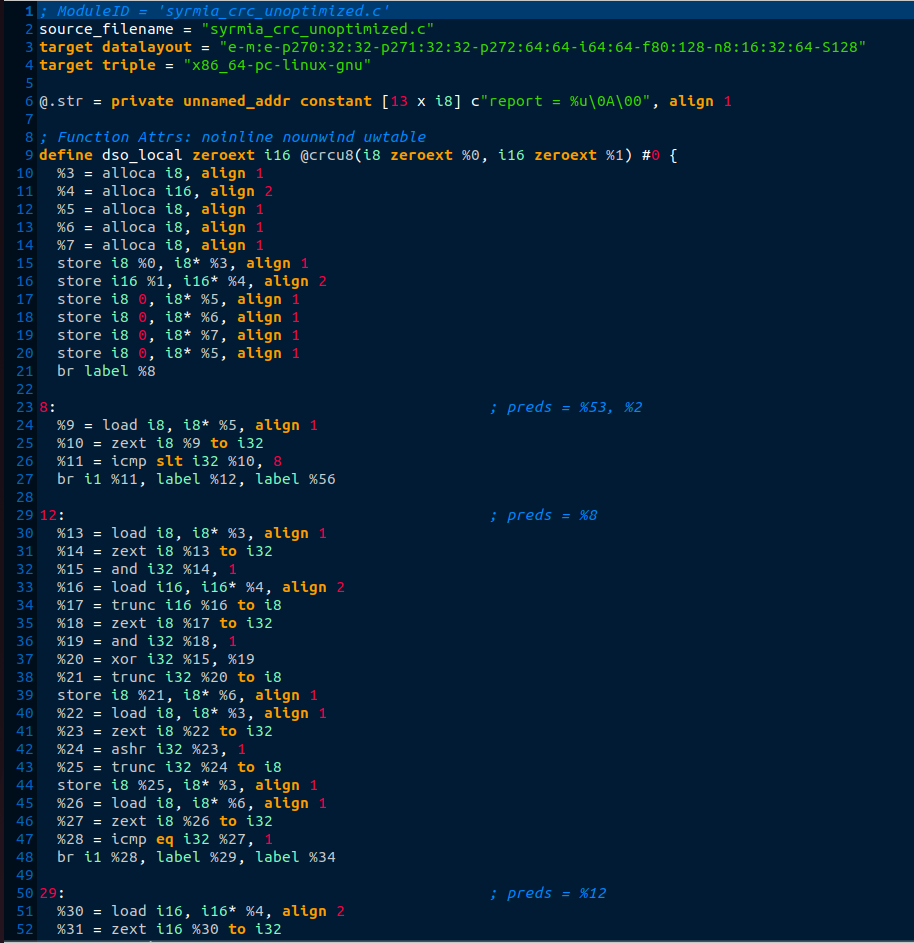
\includegraphics[width=\textwidth, height=16cm]{unoptimized_ir}
\caption{Deo fajla syrmia\_crc\_unoptimized.ll}
\centering
\end{figure}

\begin{figure}
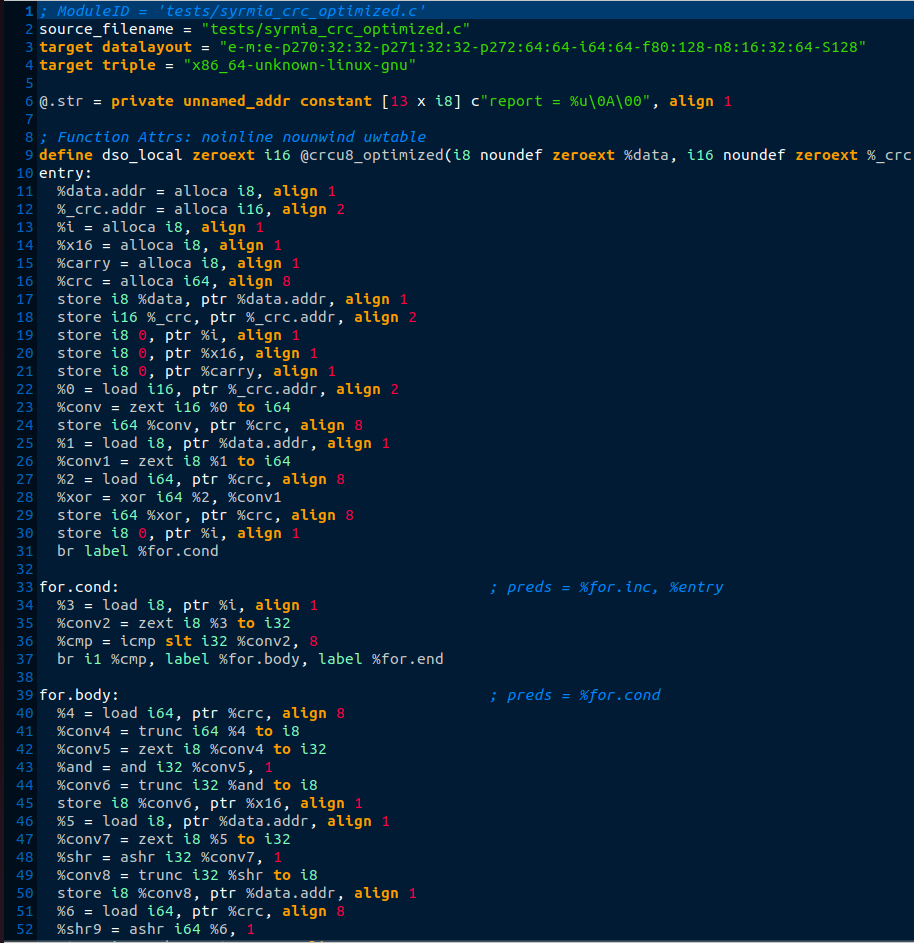
\includegraphics[width=\textwidth, height=16cm]{optimized_ir}
\caption{Deo fajla syrmia\_crc\_optimized.ll}
\centering
\end{figure}

%Implementacija 1
Prva implementacija je u potpunosti sprovedena na IR-nivou. To znači da je 
program napisan u programskim jezicima C ili C++ preveden prednjim delom LLVM 
kompilatora odnosno alatom Clang u fajl sa .ll ekstenzijom koji sadrži 
međureprezentaciju početnog programa i da je potom isti .ll fajl izmenjen tako 
da sadrži optimizovanu verziju CRC algoritma. Izmenjena međureprezentacija se 
potom može proslediti srednjem i zadnjem delu kompilatora kako bi se dobio 
objektni ili izvršivi fajl kako bi izvršavao ono što je izvornim kodom zadato.  
Izmena međureprezentacije podrazumeva prepoznavanje jedne neoptimizovane 
verzije CRC algoritma, zatim uklanjanje odnosno brisanju prepoznatih 
instrukcija i na kraju generisanju novih IR instrukcija koje pripadaju 
optimozovanoj verziji CRC algoritma. Time, dakle, od jedne sintaksno ispravne 
verzije .ll fajla dobijamo novi, takođe ispravan, .ll fajl.

Kod koji izvršava sve što je upravo ovjašnjeno nalazi se u okviru 
RecognizingCRC.cpp fajla. Gledano iz perspektive LLVM arhitekture ove provere 
predstavljaju optimizacioni prolaz pod nazivom crc-recognition. Samo 
prepoznavanje algoritma izvršeno je kretanjem unazad kroz instrukcije svake od 
funckija u .ll fajlu odnosno modulu koji obrađujemo. Kretanje započinjemo od 
poslednje instrukcije poslednjeg osnovnog bloka i krećemo se unazad po 
prethodnim instrukcijama poslednjeg bazičnog bloka, a zatim i po instrukcijama 
prethodnih bazičnih blokova, sve dok ne dođemo do prvi instrukcije u prvom 
bazičnom bloku. U svakom koraku proveravamo da li smo naišli na instrukciju 
koju očekujemo i proveramo da li je instrukcija pozvana nad odgovarajućim 
virtuelnim registrima odnosno operandima. Ukoliko u bilo kom koraku primetimo 
razliku bilo u instrukciji koju proveravamo bilo u njenim operandima, 
završavamo sa izvršavanjem naše funkcije vraćanjem false povratne vrednosti. 
Time signaliziramo da algoritam od našeg interesa nije prepoznat. U protivnom, 
ukoliko do prekida funkcije za proveru nije došlo (i ukoliko je i poslednja 
instrukcija proverena) zaključujemo da smo prepoznali traženi algoritam i da 
možemo započeti brisanje prepoznatih instrukcija. 

Brisanje prepoznatih instrukcija takođe izvršavamo kretanjem unazada i uklanjanjem svake od instrukcija na koju naiđemo. Iako je prepoznavanje algoritma moglo biti izvršeno i u suprotnom smeru odnosno kretanjem unapred od prve ka poslednjoj instrukciji, brisanje instrukcija neke funkcije je ipak bolje obaviti kretanjem u nazad. Razlog za tako nešto jesto to što su "kasnije" instrukcije (instrukcije bliže poslednjoj) dosta zavisne od "bližih" instrukcija....

Nakon uspešnog brisanja prepoznatih instrukcija, generišemo instrukcije koje pripadaju međukodu optimizovanog CRC algoritma i to radimo kreiranjem prvog bazičnog bloka, zatim drugog i sve tako do poslednjeg. Dakle, da rezimiramo, prepoznavanje i uklanjanje prepoznatih instrukcija su u obe implementacije izvršene kretanjem u nazad, dok je generisanje novih instrukcija izvršeno kretanjem unapred. 

%Implementacija 2
Druga implementacija je u velikoj meri slična prvoj, ali su im se vaze generisanja optimizovanog koda bitnog razlikuju. Dakle, druga implementacija takođe počiva na prepoznavanju jedne neoptimizovane varijante CRC algoritma, i zatim uklanjanju prepoznatih istrukcija. 
Međutim, nakon uklanjanja prepoznatih instrukcija druga implementacija predlaže kreiranje poziva intrinzičke funkcije pod nazivom riscv-crc i korišćenje povratne vrednosti te funkcije kao povratne vrednosti funkcije čiji smo kod upravo prepoznali i obrisali. Argumenti intrinzičke funkcije su identični argumentima funkcije čiji kod prepoznajemo. 
potom kreiranju poziva. Pred sam kraj prevođenja programa 
intrinzička funkcija se zamenjuje sekvencom mašinskih instrukcija koje pripadaju optimizovanoj varijanti CRC algoritma. 

Pojam intrinzičke funkcije (engl. intrinsic function) jeste termin koji se obilato koristi oko projekta LLVM, ali 
za koji ne postoji tačna definicija. Intrinzička funkcija bi trebalo da 
predstavlja funkciju koja se kroz veći deo LLVM pipeline-a može smatrati 
validnom iako nikakav kod ne postoji iza nje, ali koja će u određenjom trenutku 
biti zamanjena blokom koda koji bi trebalo da predstavlja.  

Da bi neka funkcija bila deklarisana kao intrinzička funkcija, potrebno je istu deklarisati u okviru posebnih fajlova projekta LLVM. Ti su fajlovi sa ekstenzijom .td unutar kojih je sadržaj napisan domenski specifičnim jezikom TableGen.

TableGen fajl pokrivaju značajan procenat celokupnog kodu u okviru LLVM projekta. Ukoliko pozovete alat cloc (akronim od Count Line Of Code) videćete da je više od 500 000 linija koda ispisano upravo u TableGen-u. 

Svaki .ll fajl u okviru projekta LLVM odgovara tačno jednom modulu. Svaki modul se sastoji od funkcija i drugih atributa. Ukoliko pristupimo funckiji nekog modula time smo zapravo pristupili funckiji napisanoj u našem izvornom kodu.

Obe implementacije su dodate u projekat LLVM kao optimizacioni prolaz na nivou 
međureprezentacije (IR nivou). Naziv optimizacionog prolaza je crc-recognition.
Obe implementacije su prvobitno bile deo optimizacionog prolaza pod imenom 
aggressive-instcombine koji je opisan u fajlovima AggressiveInstCombine.cpp i 
AggressiveInstCombine.h.

Trebalo bi reći nešto više o drugoj modifikaciji napravljenoj u TableGen-u. 

Na kraju, trebalo bi malo bolje opisati drugo implementaciono rešenje, odnosno 
osvrnuti se na korake koju su bili preduzeti kako bi se rešenje do kraja 
sprovelo. Naime, bilo je potrebno već spomenutu intrinzičku funkciju llvm.crc32 
deklarisati u još nekim TableGen fajlovima kako bi intrinzička funkcija mogla 
proći kroz faze LLVM backend-a. Ponovna deklaracija u TableGen-u ima za cilj 
prevođenje validnog SelectionDAG čvora predstavljenog kreiranom llvm.crc 
intrinzičkom funkcijom u pseudo mašinsku instrukciju. Ta pseudo mašinska 
instrukcija se potom propagira kroz LLVM pipeline i u nekom momentu zamenjuje 
sekvencom tačno određenih mašinskih instrukcija izvršivih na procesorskoj 
arhitekturi RISC-V. Motivacija za korišćenje određene sekvence mašinskih instrukcija 
u ovom implementacionom rešenju biće objašnjeno u narednom poglavlju.
% ------------------------------------------------------------------------------
\chapter{Rezultati implementacije}
% ------------------------------------------------------------------------------
U ovom poglavlju biće predstavljeni rezultati dobijeni pokretanjem oba implementaciona rešenja 
predstavljena u prethodnom poglavlju. Za potrebe testiranja rezultata prvog implementacionog 
rešenja dovoljno je pokrenuti alat clang, a zatim LLVM optimizator (alat opt). Za 
testiranje drugog implementacionog rešenja trebalo bi pored alata clang i opt, koji se u ovom 
slučaju prevode sa nešto drugačijim argumentima, pokrenuti i alat llc koji predstavlja zadnji deo 
LLVM kompajlera (LLVM backend).  

Za testiranje prvog implementacionog rešenja potrebno je pokrenuti komande prikazane na slici 6.1.
Prvom komandom se program napisan u programskom jeziku C (sadržan u fajlu 
syrmia-crc-unoptimized.c) se prevodi u LLVM međureprezentaciju upotrebom prednjeg dela LLVM 
kompilatora odnosno alata Clang. Drugom komandom se pokreće LLVM optimizator, to jest, alat opt 
kojim se započinju analize i transformacije međukoda dobijenog pozivom prethodne komande. Kao 
rezultat poziva ove komande dobija se optimizovana LLVM međureprezentacija iliti optimizovani 
LLVM međukod. 

\begin{figure}
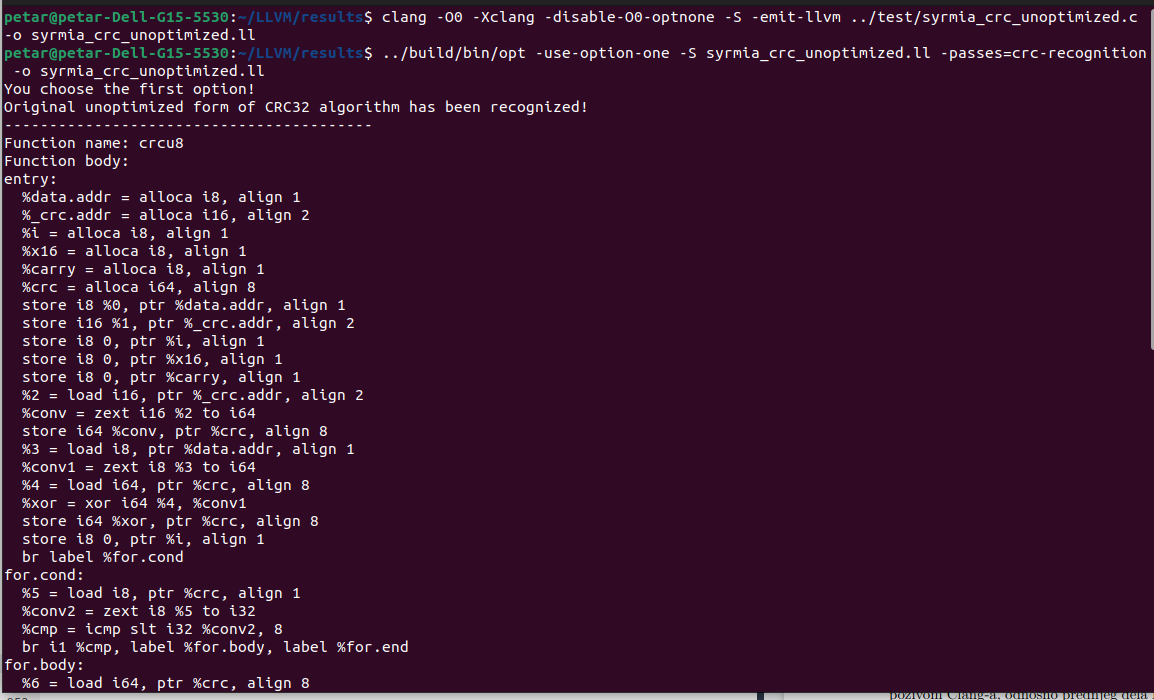
\includegraphics[width=\textwidth, height=12cm]{testing_1st_impl}
\caption{Pokretanje prvog implementacionog rešenja}
\end{figure}

Opcijama "-S" i "-emit-llvm" navedenim u prvoj komandi se naglašava da je ulazni fajl potrebno 
prevesti u LLVM međureprezentaciju. Opcija "-disable-O0-optnone" takođe navedena u prvoj komandi 
služi da omogući da eventualni poziv LLVM optimizatora nad izlaznim fajlom (fajlom dobijenim 
pozivom prve komande) može da sprovede transformacije nad LLVM međukodom. Što se tiče druge 
komande, u njoj se navedene opcije "-S", "-passes" i "-use-option-one". Opcijom "-S" naglašavamo 
da je izlazni fajl potrebno predstaviti LLVM međureprezentacijom, a ne bajtkodom (engl. 
bytecode). Opcijom "-passes=" biramo optimizacioni prolaz koji želimo da pokrenemo. U prethodnom 
poglavlju je naglašeno da se oba implementaciona rešenja nalaze u okviru "crc-recognition" 
optimizacionog prolaza i zato je isti sada bio izabran. Na kraju, opcija "-use-option-one" nije 
podrazumevana opcija za LLVM optimizator iliti alat opt već je to korisnički definisana opcija. 
Tom opcijom se u crc-recognition optimizacionom prolazu naglašava da je potrebno upotrebiti prvo 
implementaciono rešenje. Na slici 6.2. možete videti sintaksnu potrebnu za uvođenjem nove opcije za LLVM optimizator.

\begin{figure}
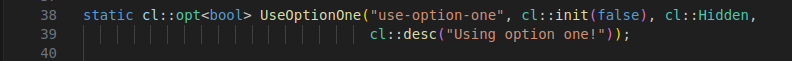
\includegraphics[width=\textwidth, height=2cm]{use_option_one}
\caption{Uvođenje korisnički definisane opcije za LLVM optimizator}
\end{figure}

Time zapravo dobijamo i potvrdu da predloženo rešenje nikako nije uzaludno.
Rezultat prevođenja prvog implementacionog rešenja se može videti pokretanje LLVM optimizatora 
(alata opt). Njegovim pokretanjem prosleđeni .ll fajl (dobijan pozivom Clang-a, odnosno prednjeg 
dela LLVM) će biti prepravljen tako da sadrži optimizovan međukod. Sadržaj tog fajla se potom 
može uporediti pozivom diff komande sa međukodom dobijenim od syrmia-crc-optimized.c fajla.

Za testiranje drugog implementacionog rešenja potrebno je pokrenuti komande prikazane na slici 
6.3. Prva komanda ima istu svrhu kao i odgovarajuća prva komanda za pokretanje prvog 
implementacionog rešenja. Ponovimo, ta svrha je da se izvorni kod prevere u oblik LLVM 
međureprezentacije. Jedina razlika sa prethodnom prvom komandom jesu dve dodatne opcije i to su: 
"-target" i "-march". Opcijom "target" bira se uopštena konfiguracija procesora na kome želimo da 
se krajnji mašinski kod izvršava. Opcija "-march" služi za dodavanje specifičnih atributa o već 
odabranom procesoru. Vrednost "rv64izbc" predstavlja posebnu verziju RISC-V procesora širine 64 bita koji nam omogućava korišćenje preko nam potrebne instrukcije clmul.

Drugom komandom se, kao i u slučaju prvog rešenja, pokreće LLVM optimizator (alat opt) koji bi 
trebalo da sprovede optimizacione alaze i transformacije nad fajlom dobijem iz prve (prethodne) 
komande. Opcijom "-passes" ponovo biramo crc-recognition optimizacioni prolaz, ali ovoga puta 
biramo opciju "-use-option-two". Njom naglašavamo da eventualno prepoznati CRC algoritam bude 
obrađen na osnovu drugog implementacionog rešenja.

Trećom komandom se poziva zadnji deo LLVM kompajlera (alat llc) sa dodatnim opcijama kao što su 
-print-after-all i -debug. Opcija -print-after-all omogućava ispis stanja posle svakog IR i MIR 
prolaza, ali ne omogućava ispis međustanja vezana za SelectionDAG. Za tako nešto je potrebno 
dadati opciju -debug. 
Pokretanjem treće komande u fajlu out.txt će se nalaziti detaljan prikaz rada zadnjeg dela LLVM 
kompajlera. Na samom kraju tog izveštaja biće ostavljen asemblerski kod spreman za izvršavanje na 
odabranoj arhitekturi. Prikaz izveštaja dobijenog na osnovu drugog implementacionog rešenja 
možete videti u nastavku...

\begin{figure}
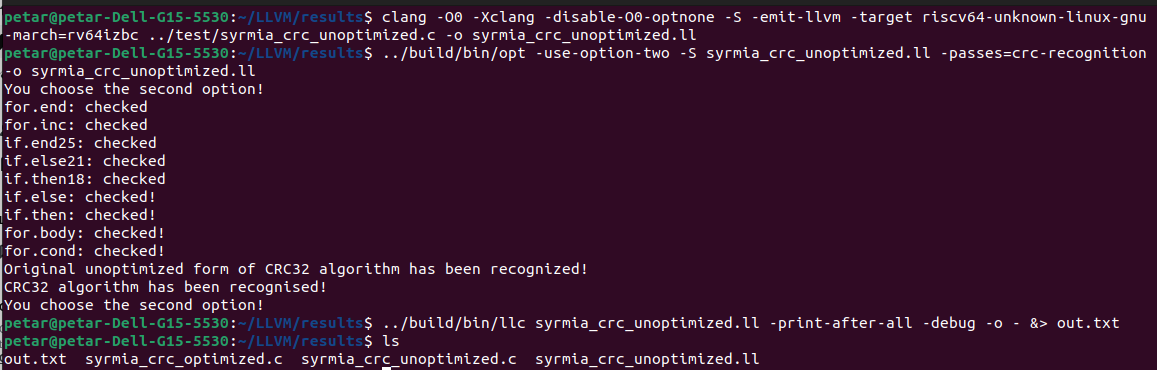
\includegraphics[width=\textwidth, height=7cm]{testing_2nd_impl}
\caption{Pokretanje drugog implementacionog rešenja}
\end{figure}

%Komande koje je potrebno pokrenuti kako bi rezultati optimizacionog prolaza opisanog u radu bili prikazani: 

%1) build/bin/clang -O0 -Xclang -disable-O0-optnone -S -emit-llvm -target riscv64-unknown-linux-gnu -march=rv64izbc tests/syrmia_crc_unoptimized.c -o syrmia_crc_unoptimized.ll

%2) build/bin/opt -use-opt-one -S tests/syrmia_crc_unoptimized.ll -passes=aggressive-instcombine -o syrmia_crc_unoptimized.ll

%3) build/bin/llc syrmia_crc_unoptimized.ll -print-after-all -debug -o - &> out.txt

Dobijeni asemblerski kod se podudara sa asemblerskim kodom navedenim u patch-u 
koji je korišćen kao resurs. U spomenutom patch-u je predstavljena podrška za 
efikasnije prevođenje algoritma CRC u okviru kompajlera GCC, a za kasnije 
korišćenje odnosno izvršavanje na RISC-V arhitekturi. Patch možete pronaći na 
sledećem linku: \url{https://www.mail-archive.com/gcc-patches@gcc.gnu.org/
msg315381.html}.

Kako se kao izlaz alata llc dobija asemberski kod za procesorsku arhitekturu RISC-V, a mašina na 
kojoj je čitav proces prevođenja izvršen pripada CISC arhitekturi procesora, potrebno je dobijeni 
mašinski kod izvršiti na nekom od emulatora. Na primer, neka to bude na emulatoru QEMU\cite{qemu}.

QEMU predstavlja program koji je u stanju da simuliranja izvršavanje operativnog sistema i 
programa za jednu mašinu na drugoj mašini. Pod mašinom podrazumevamo računarski sistem sa 
procesorskom arhitekturom prisutnom na njemu.

Iako je pojam cross kompajliranja već implicitno objašnjen, nije na odmet da i eklpicitno bude 
objašnjen. Cross kompajliranje (engl. cross compiling) predstavlja proces prevođenja programa i 
kreiranja mašinskog koda za jednu mašinu koja je potencijalno drugačija od mašine na kojoj je i
izvršen proces prevođenja.

Dakle, potrebno je objektni ili izvršni fajl proslediti emulatoru QEMU kako bismo simulirali 
izvršavanje našeg početnog programa na arhitekturi RISC-V. 
Jedini problem na koji nailazimo nakon poziva alata llc jeste to što kao rezultat njegovog rada 
dobijamo ili mašinski kod ili objektni fajl (naravno, u zavisnosti od opcija koje odaberemo 
prilikom njegovog pokretanja). Objektni fajl i fajl sa mašinskim kodom još uvek ne predstavljaju 
izvršne fajlove, što znači da je potrebno pozvati linker koji bi od objektnih fajlova kreirao 
izvršnu datoteku. U ovom slučaju to može biti Clang.

Treblo bi napomenuti da trenutna implementacija funkcioniše samo za pristup odabiru instrukcija 
ostvarenom kroz SelectionDAG. Iako to za sada deluje u redu, u budućnosti  bi trebalo podržati 
GlobalIsel pristup selekcije instrukcija koji se sve više koristi.

Za obe implementacije napravljen je određen broj regresionih testova koji proveravaju da li je 
algoritam CRC uspešno prepoznat i zamenjen drugom verzijom algoritma.

Za testiranje promena napravljenih u okviru LLVM kompajlera kreirana je čitava infrastruktura za 
testiranje. LLVM infrastruktura za testiranje omogućava korišćenje testova jedinica koda (engl 
unit tests), regresionih testova, kao i čitavih programa za testiranje. Regresioni i unit testovi 
su već sadržani u LLVM-ovom repozitorijumu u okviru foldera llvm/test i llvm/unittests. Očekuje 
se da svaki od ovih testova prolazi tako da je preporuka pokrenuti ih pre bilo kreiranja bilo kog 
commit-a.

Čitavi programi za testiranje se nazivaju "LLVM test suite" ili samo "test-suite" i za njih 
postoji čitav repozitorijum na platformi GitHub. Iz istorijskih razloga, ovi testovi se na nekim 
mestima nazivaju i "nightly tests", što je više određenije u odnosu na "test-suite". 

Testovi jedinica koda iliti unit testovi su napisani korišćenjem Google testova i Google Mock-a, 
kao što je već rečeno, nalaze se u llvm/unittests direktorijumu. Unit testovi se koriste za 
proveru korišćenja biblioteka i za druge generičke strukture podataka. Ukoliko je potrebno 
testirati transformacije i analize sprovedene na nivou međureprezentacije, odnosno IR nivou, u 
tom slučaju je bolje koristiti regresione testove.

Regresioni testovi su mali delovi koda koji testiraju specifičnu komponentu LLVM kompajlera ili 
trigeruju odnosno izazivaju određeni bag u okviru LLVM-a. Jezik u kome su napisani zavisi od dela 
LLVM-a koji se tim testom proverava. Regresioni testovi se nalaze u okviru direktorijuma 
llvm/test i pokreću se alatom llvm-lit koji takođe predstavlja deo projeta LLVM.

Obično kada se pronađe neki bug u okviru projekta LLVM, regresioni testovi bi trebalo da sadrže 
taman dovoljno koda da reprodukuju problem i trebalo bi da se nalaze negde u okviru llvm/test 
direktorijuma. Na primer, regresioni test može biti mali deo LLVM IR-a izdvojen iz neke 
aplikacije ili benchmark statistika (benchmark).

Testirajuće analize predstavljaju LLVM prolaze koji izdvode zaključke o kvalitetu LLVM IR-a, ali 
ga ne transformišu. Ove analize su testirane korišćenjem iste infrastrukture kao i regresioni 
testovi, odnosno kreiranjem odvojenog "Printer" prolaza kako bi se rezultati analiza iskoristili 
i ispisali na standardni izlaz u vidu tekstualnog formata prilagođenog alatu FileCheck.
Predlažem da pogledate llvm/test/Analysis/BranchProbabilityInfo/loop.ll za primere takvih testova.

Promene se opisane u ovom radu biće testirane kreiranjem regresionih testova, a potom pokretanjem alata llvm-lit i Filecheck nad njima.

Alat llvm-lit...

Alat Filecheck...
Alat Filecheck čita dva fajla (jedan sa standardnog ulaza, a jedan naveden kao argument komandne linije) i koristi jedan kako bi verifikovao drugi. Ovakvo ponašanje je izuzetno korisno za pokretanje testsuite-a, koji pokušava da proveri da li rezultat rada nekog alata (na primer alata llc) sadrži neku očekivanu informaciju (na primer instrukciju clmul u asemblerskom kodu koji alat generiše). Deluje je da je alat Filecheck vrlo sličan alatu grep, međutim alat Filecheck omogućava daleko efikasnije prepoznavanje više različitih ulaza u jednom fajlu i izlistavanje prepoznatih delova u specifičnom redosledu. 

Uputstvo za korišćenje alata Filecheck izgleda ovako:
\begin{lstlisting}[language=bash]
FileCheck match-filename [–check-prefix=XXX] [–strict-whitespace]
\end{lstlisting}

Fajl match-filename predstavlja fajl koji sadrži obrazac koji treba prepoznati. Fajl koji se verifkuje se unosi sa standardnog ulaza ukoliko opcija --input-file nije upotrebljena.

%Možemo uporediti vremena izvršavanja oba verzije algoritma nad ulazom veličine milijardu. U tom slučaju dobijamo razliku od 2 sekunde u korist optimizovane verzije CRC algoritma. U nastavku je prikazen test koji smo sproveli, kao i rezultati tog testa...

Poređenjem rezultata dobijenih pokretanjem neoptimizovane verzije CRC algoritma i semantički 
ekvivalentne optimizovane verzije nad ulazom veličine milijardu zaključujemo da je optimizovana 
verzija daleko efikasnija. Razlika ove dve verzije algortima je u nekim slučajevima čak 6 sekundi 
u korist optimizovane verzije algoritma CRC. Jedan od rezultata dobijenih upoređivanjem možete 
videti u nastavku.

\begin{figure}
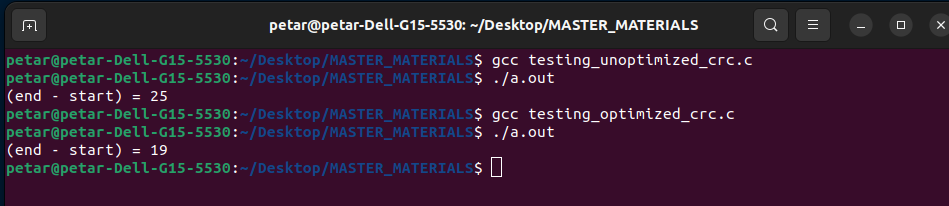
\includegraphics[width=\textwidth, height=4cm]{comparing_crcs}
\caption{Rezultat upoređivanja optimizovane i neoptimizovane verzije algoritma CRC nad ulazom veličine milijardu}
\end{figure}

Sadržaj fajla testing-uoptimized-crc.c izgleda ovako:
\begin{figure}
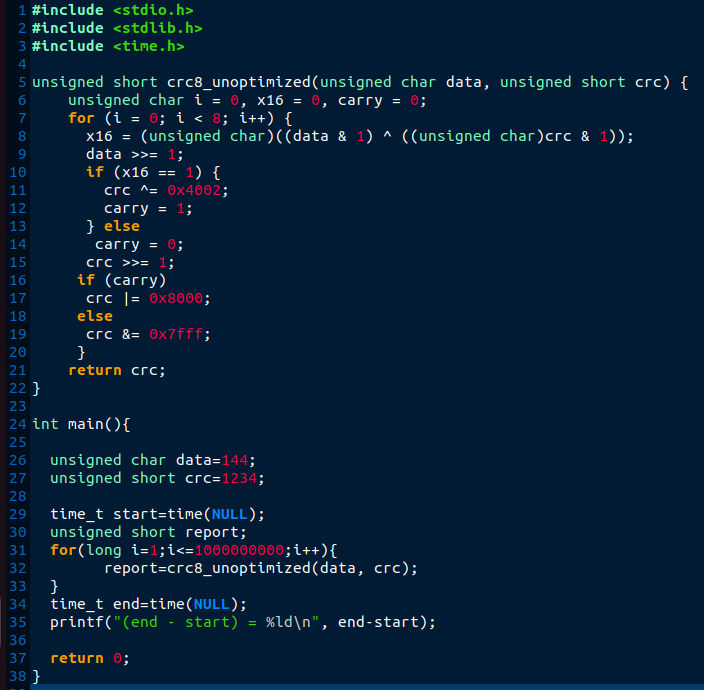
\includegraphics[width=\textwidth, height=12cm]{testing_unoptimized_crc}
\caption{Sadržaj fajla testing\_unoptimized\_crc.c}
\end{figure}

Sadržaj fajla testing-optimized-crc.c izgleda ovako:
\begin{figure}
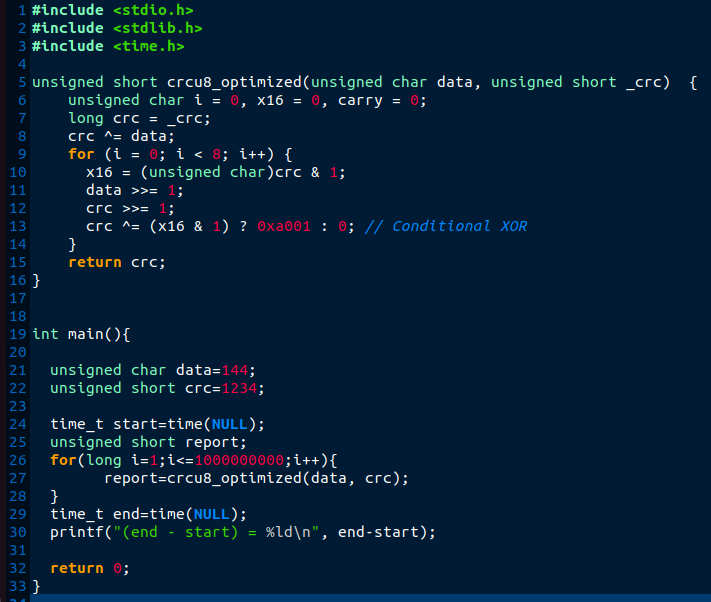
\includegraphics[width=\textwidth, height=12cm]{testing_optimized_crc}
\caption{Sadržaj fajla testing\_optimized\_crc.c}
\end{figure}

\cite{stulova2019overview}
\cite{lit}
\cite{llvm}
\cite{lit}
% ------------------------------------------------------------------------------
\chapter{Zaključak}
% ------------------------------------------------------------------------------
U ovom radu predstavljeno je sledeće...

Nadam se da će ovaj rad dati motivaciju i smernice za unapređivanje LLVM i drugih kompajlera kako 
bi se i neki drugi algoritmi, aritmetički izrazi ili često korišćene programske konstrukcije 
efikasnije prevodile.
% ------------------------------------------------------------------------------
% Literatura
% ------------------------------------------------------------------------------
\literatura

% ==============================================================================
% Završni deo teze i prilozi
\backmatter
% ==============================================================================

% ------------------------------------------------------------------------------
% Biografija kandidata
\begin{biografija}
%(\emph{Beograd, 19. јул 1999.})
\textbf{Petar Tešić}  je rođen 19. jula 1999. godine u Beogradu. Osnovnu školu i opšti smer gimnazije završio je u Ubu. Nakon završene gimnazije upisao je Matematički fakultet u Beogradu na smeru Računarstvo i informatika u okviru studijskog programa Matematika. Osnovne studije završio je u roku sa prosečnom ocenom 9,25. Po završetku osnovnih studija, upisao je master studije na Matematičkom fakultetu na smeru Informatika i postao saradnik u nastavi na katedri za računarstvo i informatiku. Kao saradnik u nastavi bio je angažovan na sledećim kursevima: Programiranje 2, Uvod u relacione baze podataka, Prevođenje programskih jezika i Računarske mreže. Radio je dva meseca kao praktikant u kompaniji FIS. Nakon toga se priključio kompaniji SYRMIA kao član System Software tima gde je radio na zadatku predstavljenom u ovom radu, a takođe je bio angažovan i na internom projektu Autocheck.
\end{biografija}
% ------------------------------------------------------------------------------

\end{document} 
